% Created by tikzDevice version 0.12.6 on 2025-02-15 07:57:21
% !TEX encoding = UTF-8 Unicode
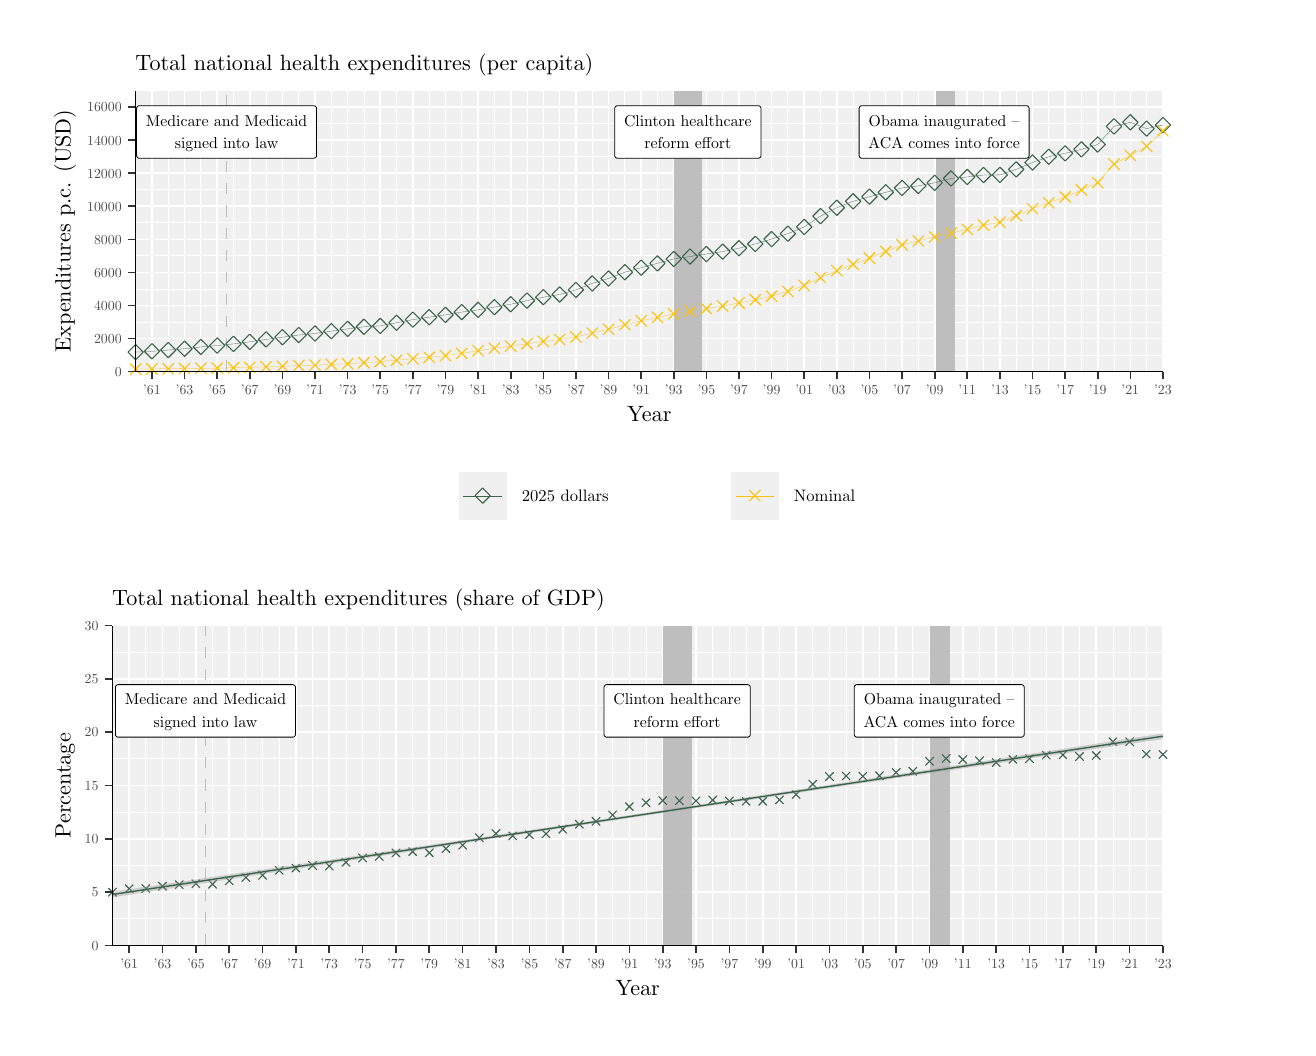
\begin{tikzpicture}[x=1pt,y=1pt]
\definecolor{fillColor}{RGB}{255,255,255}
\path[use as bounding box,fill=fillColor,fill opacity=0.00] (0,0) rectangle (455.30,361.35);
\begin{scope}
\path[clip] (  0.00,168.07) rectangle (455.30,361.35);
\definecolor{drawColor}{RGB}{255,255,255}
\definecolor{fillColor}{RGB}{255,255,255}

\path[draw=drawColor,line width= 0.6pt,line join=round,line cap=round,fill=fillColor] ( -0.00,168.07) rectangle (455.30,361.35);
\end{scope}
\begin{scope}
\path[clip] (  0.00,  0.00) rectangle (455.30,361.35);
\definecolor{fillColor}{gray}{0.94}

\path[fill=fillColor] ( 38.93,237.10) rectangle (410.30,338.57);
\definecolor{drawColor}{RGB}{255,255,255}

\path[draw=drawColor,line width= 0.3pt,line join=round] ( 38.93,243.07) --
	(410.30,243.07);

\path[draw=drawColor,line width= 0.3pt,line join=round] ( 38.93,255.01) --
	(410.30,255.01);

\path[draw=drawColor,line width= 0.3pt,line join=round] ( 38.93,266.94) --
	(410.30,266.94);

\path[draw=drawColor,line width= 0.3pt,line join=round] ( 38.93,278.88) --
	(410.30,278.88);

\path[draw=drawColor,line width= 0.3pt,line join=round] ( 38.93,290.82) --
	(410.30,290.82);

\path[draw=drawColor,line width= 0.3pt,line join=round] ( 38.93,302.76) --
	(410.30,302.76);

\path[draw=drawColor,line width= 0.3pt,line join=round] ( 38.93,314.70) --
	(410.30,314.70);

\path[draw=drawColor,line width= 0.3pt,line join=round] ( 38.93,326.64) --
	(410.30,326.64);

\path[draw=drawColor,line width= 0.3pt,line join=round] ( 38.93,338.57) --
	(410.30,338.57);

\path[draw=drawColor,line width= 0.3pt,line join=round] ( 39.02,237.10) --
	( 39.02,338.57);

\path[draw=drawColor,line width= 0.3pt,line join=round] ( 50.80,237.10) --
	( 50.80,338.57);

\path[draw=drawColor,line width= 0.3pt,line join=round] ( 62.59,237.10) --
	( 62.59,338.57);

\path[draw=drawColor,line width= 0.3pt,line join=round] ( 74.37,237.10) --
	( 74.37,338.57);

\path[draw=drawColor,line width= 0.3pt,line join=round] ( 86.15,237.10) --
	( 86.15,338.57);

\path[draw=drawColor,line width= 0.3pt,line join=round] ( 97.94,237.10) --
	( 97.94,338.57);

\path[draw=drawColor,line width= 0.3pt,line join=round] (109.72,237.10) --
	(109.72,338.57);

\path[draw=drawColor,line width= 0.3pt,line join=round] (121.51,237.10) --
	(121.51,338.57);

\path[draw=drawColor,line width= 0.3pt,line join=round] (133.29,237.10) --
	(133.29,338.57);

\path[draw=drawColor,line width= 0.3pt,line join=round] (145.08,237.10) --
	(145.08,338.57);

\path[draw=drawColor,line width= 0.3pt,line join=round] (156.86,237.10) --
	(156.86,338.57);

\path[draw=drawColor,line width= 0.3pt,line join=round] (168.65,237.10) --
	(168.65,338.57);

\path[draw=drawColor,line width= 0.3pt,line join=round] (180.43,237.10) --
	(180.43,338.57);

\path[draw=drawColor,line width= 0.3pt,line join=round] (192.21,237.10) --
	(192.21,338.57);

\path[draw=drawColor,line width= 0.3pt,line join=round] (204.00,237.10) --
	(204.00,338.57);

\path[draw=drawColor,line width= 0.3pt,line join=round] (215.78,237.10) --
	(215.78,338.57);

\path[draw=drawColor,line width= 0.3pt,line join=round] (227.57,237.10) --
	(227.57,338.57);

\path[draw=drawColor,line width= 0.3pt,line join=round] (239.35,237.10) --
	(239.35,338.57);

\path[draw=drawColor,line width= 0.3pt,line join=round] (251.14,237.10) --
	(251.14,338.57);

\path[draw=drawColor,line width= 0.3pt,line join=round] (262.92,237.10) --
	(262.92,338.57);

\path[draw=drawColor,line width= 0.3pt,line join=round] (274.70,237.10) --
	(274.70,338.57);

\path[draw=drawColor,line width= 0.3pt,line join=round] (286.49,237.10) --
	(286.49,338.57);

\path[draw=drawColor,line width= 0.3pt,line join=round] (298.27,237.10) --
	(298.27,338.57);

\path[draw=drawColor,line width= 0.3pt,line join=round] (310.06,237.10) --
	(310.06,338.57);

\path[draw=drawColor,line width= 0.3pt,line join=round] (321.84,237.10) --
	(321.84,338.57);

\path[draw=drawColor,line width= 0.3pt,line join=round] (333.63,237.10) --
	(333.63,338.57);

\path[draw=drawColor,line width= 0.3pt,line join=round] (345.41,237.10) --
	(345.41,338.57);

\path[draw=drawColor,line width= 0.3pt,line join=round] (357.19,237.10) --
	(357.19,338.57);

\path[draw=drawColor,line width= 0.3pt,line join=round] (368.98,237.10) --
	(368.98,338.57);

\path[draw=drawColor,line width= 0.3pt,line join=round] (380.76,237.10) --
	(380.76,338.57);

\path[draw=drawColor,line width= 0.3pt,line join=round] (392.55,237.10) --
	(392.55,338.57);

\path[draw=drawColor,line width= 0.3pt,line join=round] (404.33,237.10) --
	(404.33,338.57);

\path[draw=drawColor,line width= 0.6pt,line join=round] ( 38.93,237.10) --
	(410.30,237.10);

\path[draw=drawColor,line width= 0.6pt,line join=round] ( 38.93,249.04) --
	(410.30,249.04);

\path[draw=drawColor,line width= 0.6pt,line join=round] ( 38.93,260.98) --
	(410.30,260.98);

\path[draw=drawColor,line width= 0.6pt,line join=round] ( 38.93,272.91) --
	(410.30,272.91);

\path[draw=drawColor,line width= 0.6pt,line join=round] ( 38.93,284.85) --
	(410.30,284.85);

\path[draw=drawColor,line width= 0.6pt,line join=round] ( 38.93,296.79) --
	(410.30,296.79);

\path[draw=drawColor,line width= 0.6pt,line join=round] ( 38.93,308.73) --
	(410.30,308.73);

\path[draw=drawColor,line width= 0.6pt,line join=round] ( 38.93,320.67) --
	(410.30,320.67);

\path[draw=drawColor,line width= 0.6pt,line join=round] ( 38.93,332.60) --
	(410.30,332.60);

\path[draw=drawColor,line width= 0.6pt,line join=round] ( 44.91,237.10) --
	( 44.91,338.57);

\path[draw=drawColor,line width= 0.6pt,line join=round] ( 56.69,237.10) --
	( 56.69,338.57);

\path[draw=drawColor,line width= 0.6pt,line join=round] ( 68.48,237.10) --
	( 68.48,338.57);

\path[draw=drawColor,line width= 0.6pt,line join=round] ( 80.26,237.10) --
	( 80.26,338.57);

\path[draw=drawColor,line width= 0.6pt,line join=round] ( 92.05,237.10) --
	( 92.05,338.57);

\path[draw=drawColor,line width= 0.6pt,line join=round] (103.83,237.10) --
	(103.83,338.57);

\path[draw=drawColor,line width= 0.6pt,line join=round] (115.62,237.10) --
	(115.62,338.57);

\path[draw=drawColor,line width= 0.6pt,line join=round] (127.40,237.10) --
	(127.40,338.57);

\path[draw=drawColor,line width= 0.6pt,line join=round] (139.19,237.10) --
	(139.19,338.57);

\path[draw=drawColor,line width= 0.6pt,line join=round] (150.96,237.10) --
	(150.96,338.57);

\path[draw=drawColor,line width= 0.6pt,line join=round] (162.76,237.10) --
	(162.76,338.57);

\path[draw=drawColor,line width= 0.6pt,line join=round] (174.53,237.10) --
	(174.53,338.57);

\path[draw=drawColor,line width= 0.6pt,line join=round] (186.33,237.10) --
	(186.33,338.57);

\path[draw=drawColor,line width= 0.6pt,line join=round] (198.10,237.10) --
	(198.10,338.57);

\path[draw=drawColor,line width= 0.6pt,line join=round] (209.89,237.10) --
	(209.89,338.57);

\path[draw=drawColor,line width= 0.6pt,line join=round] (221.67,237.10) --
	(221.67,338.57);

\path[draw=drawColor,line width= 0.6pt,line join=round] (233.46,237.10) --
	(233.46,338.57);

\path[draw=drawColor,line width= 0.6pt,line join=round] (245.24,237.10) --
	(245.24,338.57);

\path[draw=drawColor,line width= 0.6pt,line join=round] (257.03,237.10) --
	(257.03,338.57);

\path[draw=drawColor,line width= 0.6pt,line join=round] (268.81,237.10) --
	(268.81,338.57);

\path[draw=drawColor,line width= 0.6pt,line join=round] (280.60,237.10) --
	(280.60,338.57);

\path[draw=drawColor,line width= 0.6pt,line join=round] (292.38,237.10) --
	(292.38,338.57);

\path[draw=drawColor,line width= 0.6pt,line join=round] (304.17,237.10) --
	(304.17,338.57);

\path[draw=drawColor,line width= 0.6pt,line join=round] (315.95,237.10) --
	(315.95,338.57);

\path[draw=drawColor,line width= 0.6pt,line join=round] (327.74,237.10) --
	(327.74,338.57);

\path[draw=drawColor,line width= 0.6pt,line join=round] (339.51,237.10) --
	(339.51,338.57);

\path[draw=drawColor,line width= 0.6pt,line join=round] (351.31,237.10) --
	(351.31,338.57);

\path[draw=drawColor,line width= 0.6pt,line join=round] (363.08,237.10) --
	(363.08,338.57);

\path[draw=drawColor,line width= 0.6pt,line join=round] (374.88,237.10) --
	(374.88,338.57);

\path[draw=drawColor,line width= 0.6pt,line join=round] (386.65,237.10) --
	(386.65,338.57);

\path[draw=drawColor,line width= 0.6pt,line join=round] (398.44,237.10) --
	(398.44,338.57);

\path[draw=drawColor,line width= 0.6pt,line join=round] (410.22,237.10) --
	(410.22,338.57);
\definecolor{drawColor}{RGB}{190,190,190}

\path[draw=drawColor,line width= 0.6pt,line join=round] ( 39.01,237.10) -- ( 39.01,338.57);
\definecolor{fillColor}{RGB}{190,190,190}

\path[fill=fillColor,fill opacity=0.01] (233.46,237.10) rectangle (243.67,338.57);

\path[fill=fillColor,fill opacity=0.01] (233.46,237.10) rectangle (243.67,338.57);

\path[fill=fillColor,fill opacity=0.01] (233.46,237.10) rectangle (243.67,338.57);

\path[fill=fillColor,fill opacity=0.01] (233.46,237.10) rectangle (243.67,338.57);

\path[fill=fillColor,fill opacity=0.01] (233.46,237.10) rectangle (243.67,338.57);

\path[fill=fillColor,fill opacity=0.01] (233.46,237.10) rectangle (243.67,338.57);

\path[fill=fillColor,fill opacity=0.01] (233.46,237.10) rectangle (243.67,338.57);

\path[fill=fillColor,fill opacity=0.01] (233.46,237.10) rectangle (243.67,338.57);

\path[fill=fillColor,fill opacity=0.01] (233.46,237.10) rectangle (243.67,338.57);

\path[fill=fillColor,fill opacity=0.01] (233.46,237.10) rectangle (243.67,338.57);

\path[fill=fillColor,fill opacity=0.01] (233.46,237.10) rectangle (243.67,338.57);

\path[fill=fillColor,fill opacity=0.01] (233.46,237.10) rectangle (243.67,338.57);

\path[fill=fillColor,fill opacity=0.01] (233.46,237.10) rectangle (243.67,338.57);

\path[fill=fillColor,fill opacity=0.01] (233.46,237.10) rectangle (243.67,338.57);

\path[fill=fillColor,fill opacity=0.01] (233.46,237.10) rectangle (243.67,338.57);

\path[fill=fillColor,fill opacity=0.01] (233.46,237.10) rectangle (243.67,338.57);

\path[fill=fillColor,fill opacity=0.01] (233.46,237.10) rectangle (243.67,338.57);

\path[fill=fillColor,fill opacity=0.01] (233.46,237.10) rectangle (243.67,338.57);

\path[fill=fillColor,fill opacity=0.01] (233.46,237.10) rectangle (243.67,338.57);

\path[fill=fillColor,fill opacity=0.01] (233.46,237.10) rectangle (243.67,338.57);

\path[fill=fillColor,fill opacity=0.01] (233.46,237.10) rectangle (243.67,338.57);

\path[fill=fillColor,fill opacity=0.01] (233.46,237.10) rectangle (243.67,338.57);

\path[fill=fillColor,fill opacity=0.01] (233.46,237.10) rectangle (243.67,338.57);

\path[fill=fillColor,fill opacity=0.01] (233.46,237.10) rectangle (243.67,338.57);

\path[fill=fillColor,fill opacity=0.01] (233.46,237.10) rectangle (243.67,338.57);

\path[fill=fillColor,fill opacity=0.01] (233.46,237.10) rectangle (243.67,338.57);

\path[fill=fillColor,fill opacity=0.01] (233.46,237.10) rectangle (243.67,338.57);

\path[fill=fillColor,fill opacity=0.01] (233.46,237.10) rectangle (243.67,338.57);

\path[fill=fillColor,fill opacity=0.01] (233.46,237.10) rectangle (243.67,338.57);

\path[fill=fillColor,fill opacity=0.01] (233.46,237.10) rectangle (243.67,338.57);

\path[fill=fillColor,fill opacity=0.01] (233.46,237.10) rectangle (243.67,338.57);

\path[fill=fillColor,fill opacity=0.01] (233.46,237.10) rectangle (243.67,338.57);

\path[fill=fillColor,fill opacity=0.01] (233.46,237.10) rectangle (243.67,338.57);

\path[fill=fillColor,fill opacity=0.01] (233.46,237.10) rectangle (243.67,338.57);

\path[fill=fillColor,fill opacity=0.01] (233.46,237.10) rectangle (243.67,338.57);

\path[fill=fillColor,fill opacity=0.01] (233.46,237.10) rectangle (243.67,338.57);

\path[fill=fillColor,fill opacity=0.01] (233.46,237.10) rectangle (243.67,338.57);

\path[fill=fillColor,fill opacity=0.01] (233.46,237.10) rectangle (243.67,338.57);

\path[fill=fillColor,fill opacity=0.01] (233.46,237.10) rectangle (243.67,338.57);

\path[fill=fillColor,fill opacity=0.01] (233.46,237.10) rectangle (243.67,338.57);

\path[fill=fillColor,fill opacity=0.01] (233.46,237.10) rectangle (243.67,338.57);

\path[fill=fillColor,fill opacity=0.01] (233.46,237.10) rectangle (243.67,338.57);

\path[fill=fillColor,fill opacity=0.01] (233.46,237.10) rectangle (243.67,338.57);

\path[fill=fillColor,fill opacity=0.01] (233.46,237.10) rectangle (243.67,338.57);

\path[fill=fillColor,fill opacity=0.01] (233.46,237.10) rectangle (243.67,338.57);

\path[fill=fillColor,fill opacity=0.01] (233.46,237.10) rectangle (243.67,338.57);

\path[fill=fillColor,fill opacity=0.01] (233.46,237.10) rectangle (243.67,338.57);

\path[fill=fillColor,fill opacity=0.01] (233.46,237.10) rectangle (243.67,338.57);

\path[fill=fillColor,fill opacity=0.01] (233.46,237.10) rectangle (243.67,338.57);

\path[fill=fillColor,fill opacity=0.01] (233.46,237.10) rectangle (243.67,338.57);

\path[fill=fillColor,fill opacity=0.01] (233.46,237.10) rectangle (243.67,338.57);

\path[fill=fillColor,fill opacity=0.01] (233.46,237.10) rectangle (243.67,338.57);

\path[fill=fillColor,fill opacity=0.01] (233.46,237.10) rectangle (243.67,338.57);

\path[fill=fillColor,fill opacity=0.01] (233.46,237.10) rectangle (243.67,338.57);

\path[fill=fillColor,fill opacity=0.01] (233.46,237.10) rectangle (243.67,338.57);

\path[fill=fillColor,fill opacity=0.01] (233.46,237.10) rectangle (243.67,338.57);

\path[fill=fillColor,fill opacity=0.01] (233.46,237.10) rectangle (243.67,338.57);

\path[fill=fillColor,fill opacity=0.01] (233.46,237.10) rectangle (243.67,338.57);

\path[fill=fillColor,fill opacity=0.01] (233.46,237.10) rectangle (243.67,338.57);

\path[fill=fillColor,fill opacity=0.01] (233.46,237.10) rectangle (243.67,338.57);

\path[fill=fillColor,fill opacity=0.01] (233.46,237.10) rectangle (243.67,338.57);

\path[fill=fillColor,fill opacity=0.01] (233.46,237.10) rectangle (243.67,338.57);

\path[fill=fillColor,fill opacity=0.01] (233.46,237.10) rectangle (243.67,338.57);

\path[fill=fillColor,fill opacity=0.01] (233.46,237.10) rectangle (243.67,338.57);

\path[fill=fillColor,fill opacity=0.01] (328.04,237.10) rectangle (334.93,338.57);

\path[fill=fillColor,fill opacity=0.01] (328.04,237.10) rectangle (334.93,338.57);

\path[fill=fillColor,fill opacity=0.01] (328.04,237.10) rectangle (334.93,338.57);

\path[fill=fillColor,fill opacity=0.01] (328.04,237.10) rectangle (334.93,338.57);

\path[fill=fillColor,fill opacity=0.01] (328.04,237.10) rectangle (334.93,338.57);

\path[fill=fillColor,fill opacity=0.01] (328.04,237.10) rectangle (334.93,338.57);

\path[fill=fillColor,fill opacity=0.01] (328.04,237.10) rectangle (334.93,338.57);

\path[fill=fillColor,fill opacity=0.01] (328.04,237.10) rectangle (334.93,338.57);

\path[fill=fillColor,fill opacity=0.01] (328.04,237.10) rectangle (334.93,338.57);

\path[fill=fillColor,fill opacity=0.01] (328.04,237.10) rectangle (334.93,338.57);

\path[fill=fillColor,fill opacity=0.01] (328.04,237.10) rectangle (334.93,338.57);

\path[fill=fillColor,fill opacity=0.01] (328.04,237.10) rectangle (334.93,338.57);

\path[fill=fillColor,fill opacity=0.01] (328.04,237.10) rectangle (334.93,338.57);

\path[fill=fillColor,fill opacity=0.01] (328.04,237.10) rectangle (334.93,338.57);

\path[fill=fillColor,fill opacity=0.01] (328.04,237.10) rectangle (334.93,338.57);

\path[fill=fillColor,fill opacity=0.01] (328.04,237.10) rectangle (334.93,338.57);

\path[fill=fillColor,fill opacity=0.01] (328.04,237.10) rectangle (334.93,338.57);

\path[fill=fillColor,fill opacity=0.01] (328.04,237.10) rectangle (334.93,338.57);

\path[fill=fillColor,fill opacity=0.01] (328.04,237.10) rectangle (334.93,338.57);

\path[fill=fillColor,fill opacity=0.01] (328.04,237.10) rectangle (334.93,338.57);

\path[fill=fillColor,fill opacity=0.01] (328.04,237.10) rectangle (334.93,338.57);

\path[fill=fillColor,fill opacity=0.01] (328.04,237.10) rectangle (334.93,338.57);

\path[fill=fillColor,fill opacity=0.01] (328.04,237.10) rectangle (334.93,338.57);

\path[fill=fillColor,fill opacity=0.01] (328.04,237.10) rectangle (334.93,338.57);

\path[fill=fillColor,fill opacity=0.01] (328.04,237.10) rectangle (334.93,338.57);

\path[fill=fillColor,fill opacity=0.01] (328.04,237.10) rectangle (334.93,338.57);

\path[fill=fillColor,fill opacity=0.01] (328.04,237.10) rectangle (334.93,338.57);

\path[fill=fillColor,fill opacity=0.01] (328.04,237.10) rectangle (334.93,338.57);

\path[fill=fillColor,fill opacity=0.01] (328.04,237.10) rectangle (334.93,338.57);

\path[fill=fillColor,fill opacity=0.01] (328.04,237.10) rectangle (334.93,338.57);

\path[fill=fillColor,fill opacity=0.01] (328.04,237.10) rectangle (334.93,338.57);

\path[fill=fillColor,fill opacity=0.01] (328.04,237.10) rectangle (334.93,338.57);

\path[fill=fillColor,fill opacity=0.01] (328.04,237.10) rectangle (334.93,338.57);

\path[fill=fillColor,fill opacity=0.01] (328.04,237.10) rectangle (334.93,338.57);

\path[fill=fillColor,fill opacity=0.01] (328.04,237.10) rectangle (334.93,338.57);

\path[fill=fillColor,fill opacity=0.01] (328.04,237.10) rectangle (334.93,338.57);

\path[fill=fillColor,fill opacity=0.01] (328.04,237.10) rectangle (334.93,338.57);

\path[fill=fillColor,fill opacity=0.01] (328.04,237.10) rectangle (334.93,338.57);

\path[fill=fillColor,fill opacity=0.01] (328.04,237.10) rectangle (334.93,338.57);

\path[fill=fillColor,fill opacity=0.01] (328.04,237.10) rectangle (334.93,338.57);

\path[fill=fillColor,fill opacity=0.01] (328.04,237.10) rectangle (334.93,338.57);

\path[fill=fillColor,fill opacity=0.01] (328.04,237.10) rectangle (334.93,338.57);

\path[fill=fillColor,fill opacity=0.01] (328.04,237.10) rectangle (334.93,338.57);

\path[fill=fillColor,fill opacity=0.01] (328.04,237.10) rectangle (334.93,338.57);

\path[fill=fillColor,fill opacity=0.01] (328.04,237.10) rectangle (334.93,338.57);

\path[fill=fillColor,fill opacity=0.01] (328.04,237.10) rectangle (334.93,338.57);

\path[fill=fillColor,fill opacity=0.01] (328.04,237.10) rectangle (334.93,338.57);

\path[fill=fillColor,fill opacity=0.01] (328.04,237.10) rectangle (334.93,338.57);

\path[fill=fillColor,fill opacity=0.01] (328.04,237.10) rectangle (334.93,338.57);

\path[fill=fillColor,fill opacity=0.01] (328.04,237.10) rectangle (334.93,338.57);

\path[fill=fillColor,fill opacity=0.01] (328.04,237.10) rectangle (334.93,338.57);

\path[fill=fillColor,fill opacity=0.01] (328.04,237.10) rectangle (334.93,338.57);

\path[fill=fillColor,fill opacity=0.01] (328.04,237.10) rectangle (334.93,338.57);

\path[fill=fillColor,fill opacity=0.01] (328.04,237.10) rectangle (334.93,338.57);

\path[fill=fillColor,fill opacity=0.01] (328.04,237.10) rectangle (334.93,338.57);

\path[fill=fillColor,fill opacity=0.01] (328.04,237.10) rectangle (334.93,338.57);

\path[fill=fillColor,fill opacity=0.01] (328.04,237.10) rectangle (334.93,338.57);

\path[fill=fillColor,fill opacity=0.01] (328.04,237.10) rectangle (334.93,338.57);

\path[fill=fillColor,fill opacity=0.01] (328.04,237.10) rectangle (334.93,338.57);

\path[fill=fillColor,fill opacity=0.01] (328.04,237.10) rectangle (334.93,338.57);

\path[fill=fillColor,fill opacity=0.01] (328.04,237.10) rectangle (334.93,338.57);

\path[fill=fillColor,fill opacity=0.01] (328.04,237.10) rectangle (334.93,338.57);

\path[fill=fillColor,fill opacity=0.01] (328.04,237.10) rectangle (334.93,338.57);

\path[fill=fillColor,fill opacity=0.01] (328.04,237.10) rectangle (334.93,338.57);

\path[draw=drawColor,line width= 0.6pt,dash pattern=on 4pt off 4pt ,line join=round] ( 71.87,237.10) -- ( 71.87,338.57);
\definecolor{drawColor}{RGB}{0,0,0}
\definecolor{fillColor}{RGB}{255,255,255}

\path[draw=drawColor,line width= 0.3pt,line join=round,line cap=round,fill=fillColor] ( 40.38,314.17) --
	(103.36,314.17) --
	(103.32,314.17) --
	(103.48,314.17) --
	(103.64,314.21) --
	(103.80,314.27) --
	(103.94,314.35) --
	(104.07,314.45) --
	(104.18,314.58) --
	(104.27,314.72) --
	(104.33,314.87) --
	(104.37,315.03) --
	(104.39,315.19) --
	(104.39,315.19) --
	(104.39,332.11) --
	(104.39,332.11) --
	(104.37,332.27) --
	(104.33,332.43) --
	(104.27,332.58) --
	(104.18,332.72) --
	(104.07,332.85) --
	(103.94,332.95) --
	(103.80,333.04) --
	(103.64,333.09) --
	(103.48,333.13) --
	(103.36,333.13) --
	( 40.38,333.13) --
	( 40.51,333.13) --
	( 40.34,333.13) --
	( 40.18,333.11) --
	( 40.02,333.07) --
	( 39.87,333.00) --
	( 39.73,332.90) --
	( 39.61,332.79) --
	( 39.51,332.66) --
	( 39.44,332.51) --
	( 39.38,332.35) --
	( 39.36,332.19) --
	( 39.35,332.11) --
	( 39.35,315.19) --
	( 39.36,315.28) --
	( 39.36,315.11) --
	( 39.38,314.95) --
	( 39.44,314.79) --
	( 39.51,314.65) --
	( 39.61,314.51) --
	( 39.73,314.40) --
	( 39.87,314.30) --
	( 40.02,314.23) --
	( 40.18,314.19) --
	( 40.34,314.17) --
	cycle;
\end{scope}
\begin{scope}
\path[clip] (  0.00,  0.00) rectangle (455.30,361.35);
\definecolor{drawColor}{RGB}{0,0,0}

\node[text=drawColor,anchor=base,inner sep=0pt, outer sep=0pt, scale=  0.57] at ( 71.87,325.79) {Medicare and Medicaid };

\node[text=drawColor,anchor=base,inner sep=0pt, outer sep=0pt, scale=  0.57] at ( 71.87,317.59) { signed into law};
\end{scope}
\begin{scope}
\path[clip] (  0.00,  0.00) rectangle (455.30,361.35);
\definecolor{drawColor}{RGB}{0,0,0}
\definecolor{fillColor}{RGB}{255,255,255}

\path[draw=drawColor,line width= 0.3pt,line join=round,line cap=round,fill=fillColor] (213.16,314.17) --
	(263.96,314.17) --
	(263.92,314.17) --
	(264.09,314.17) --
	(264.25,314.21) --
	(264.40,314.27) --
	(264.55,314.35) --
	(264.68,314.45) --
	(264.79,314.58) --
	(264.87,314.72) --
	(264.94,314.87) --
	(264.98,315.03) --
	(264.99,315.19) --
	(264.99,315.19) --
	(264.99,332.11) --
	(264.99,332.11) --
	(264.98,332.27) --
	(264.94,332.43) --
	(264.87,332.58) --
	(264.79,332.72) --
	(264.68,332.85) --
	(264.55,332.95) --
	(264.40,333.04) --
	(264.25,333.09) --
	(264.09,333.13) --
	(263.96,333.13) --
	(213.16,333.13) --
	(213.28,333.13) --
	(213.12,333.13) --
	(212.95,333.11) --
	(212.79,333.07) --
	(212.64,333.00) --
	(212.51,332.90) --
	(212.39,332.79) --
	(212.29,332.66) --
	(212.21,332.51) --
	(212.16,332.35) --
	(212.13,332.19) --
	(212.13,332.11) --
	(212.13,315.19) --
	(212.13,315.28) --
	(212.13,315.11) --
	(212.16,314.95) --
	(212.21,314.79) --
	(212.29,314.65) --
	(212.39,314.51) --
	(212.51,314.40) --
	(212.64,314.30) --
	(212.79,314.23) --
	(212.95,314.19) --
	(213.12,314.17) --
	cycle;
\end{scope}
\begin{scope}
\path[clip] (  0.00,  0.00) rectangle (455.30,361.35);
\definecolor{drawColor}{RGB}{0,0,0}

\node[text=drawColor,anchor=base,inner sep=0pt, outer sep=0pt, scale=  0.57] at (238.56,325.79) {Clinton healthcare };

\node[text=drawColor,anchor=base,inner sep=0pt, outer sep=0pt, scale=  0.57] at (238.56,317.59) { reform effort};
\end{scope}
\begin{scope}
\path[clip] (  0.00,  0.00) rectangle (455.30,361.35);
\definecolor{drawColor}{RGB}{0,0,0}
\definecolor{fillColor}{RGB}{255,255,255}

\path[draw=drawColor,line width= 0.3pt,line join=round,line cap=round,fill=fillColor] (301.47,314.17) --
	(360.84,314.17) --
	(360.80,314.17) --
	(360.97,314.17) --
	(361.13,314.21) --
	(361.28,314.27) --
	(361.43,314.35) --
	(361.56,314.45) --
	(361.67,314.58) --
	(361.75,314.72) --
	(361.82,314.87) --
	(361.86,315.03) --
	(361.87,315.19) --
	(361.87,315.19) --
	(361.87,332.11) --
	(361.87,332.11) --
	(361.86,332.27) --
	(361.82,332.43) --
	(361.75,332.58) --
	(361.67,332.72) --
	(361.56,332.85) --
	(361.43,332.95) --
	(361.28,333.04) --
	(361.13,333.09) --
	(360.97,333.13) --
	(360.84,333.13) --
	(301.47,333.13) --
	(301.60,333.13) --
	(301.43,333.13) --
	(301.27,333.11) --
	(301.11,333.07) --
	(300.96,333.00) --
	(300.82,332.90) --
	(300.70,332.79) --
	(300.60,332.66) --
	(300.53,332.51) --
	(300.47,332.35) --
	(300.45,332.19) --
	(300.44,332.11) --
	(300.44,315.19) --
	(300.45,315.28) --
	(300.45,315.11) --
	(300.47,314.95) --
	(300.53,314.79) --
	(300.60,314.65) --
	(300.70,314.51) --
	(300.82,314.40) --
	(300.96,314.30) --
	(301.11,314.23) --
	(301.27,314.19) --
	(301.43,314.17) --
	cycle;
\end{scope}
\begin{scope}
\path[clip] (  0.00,  0.00) rectangle (455.30,361.35);
\definecolor{drawColor}{RGB}{0,0,0}

\node[text=drawColor,anchor=base,inner sep=0pt, outer sep=0pt, scale=  0.57] at (331.16,325.79) {Obama inaugurated -- };

\node[text=drawColor,anchor=base,inner sep=0pt, outer sep=0pt, scale=  0.57] at (331.16,317.59) { ACA comes into force};
\end{scope}
\begin{scope}
\path[clip] (  0.00,  0.00) rectangle (455.30,361.35);
\definecolor{drawColor}{RGB}{60,100,75}

\path[draw=drawColor,line width= 0.4pt,line join=round,line cap=round] ( 36.23,244.10) --
	( 39.01,246.88) --
	( 41.78,244.10) --
	( 39.01,241.33) --
	cycle;

\path[draw=drawColor,line width= 0.4pt,line join=round,line cap=round] ( 42.14,244.40) --
	( 44.91,247.18) --
	( 47.69,244.40) --
	( 44.91,241.63) --
	cycle;

\path[draw=drawColor,line width= 0.4pt,line join=round,line cap=round] ( 48.03,244.86) --
	( 50.80,247.63) --
	( 53.58,244.86) --
	( 50.80,242.08) --
	cycle;

\path[draw=drawColor,line width= 0.4pt,line join=round,line cap=round] ( 53.91,245.32) --
	( 56.69,248.10) --
	( 59.46,245.32) --
	( 56.69,242.55) --
	cycle;

\path[draw=drawColor,line width= 0.4pt,line join=round,line cap=round] ( 59.80,245.98) --
	( 62.58,248.76) --
	( 65.35,245.98) --
	( 62.58,243.21) --
	cycle;

\path[draw=drawColor,line width= 0.4pt,line join=round,line cap=round] ( 65.71,246.47) --
	( 68.48,249.25) --
	( 71.26,246.47) --
	( 68.48,243.70) --
	cycle;

\path[draw=drawColor,line width= 0.4pt,line join=round,line cap=round] ( 71.60,247.08) --
	( 74.37,249.86) --
	( 77.15,247.08) --
	( 74.37,244.31) --
	cycle;

\path[draw=drawColor,line width= 0.4pt,line join=round,line cap=round] ( 77.48,247.83) --
	( 80.26,250.60) --
	( 83.03,247.83) --
	( 80.26,245.05) --
	cycle;

\path[draw=drawColor,line width= 0.4pt,line join=round,line cap=round] ( 83.37,248.71) --
	( 86.15,251.48) --
	( 88.92,248.71) --
	( 86.15,245.93) --
	cycle;

\path[draw=drawColor,line width= 0.4pt,line join=round,line cap=round] ( 89.28,249.50) --
	( 92.05,252.27) --
	( 94.83,249.50) --
	( 92.05,246.72) --
	cycle;

\path[draw=drawColor,line width= 0.4pt,line join=round,line cap=round] ( 95.16,250.28) --
	( 97.94,253.06) --
	(100.71,250.28) --
	( 97.94,247.51) --
	cycle;

\path[draw=drawColor,line width= 0.4pt,line join=round,line cap=round] (101.05,250.84) --
	(103.83,253.62) --
	(106.60,250.84) --
	(103.83,248.07) --
	cycle;

\path[draw=drawColor,line width= 0.4pt,line join=round,line cap=round] (106.94,251.68) --
	(109.72,254.45) --
	(112.49,251.68) --
	(109.72,248.90) --
	cycle;

\path[draw=drawColor,line width= 0.4pt,line join=round,line cap=round] (112.84,252.52) --
	(115.62,255.29) --
	(118.39,252.52) --
	(115.62,249.74) --
	cycle;

\path[draw=drawColor,line width= 0.4pt,line join=round,line cap=round] (118.73,253.27) --
	(121.51,256.05) --
	(124.28,253.27) --
	(121.51,250.50) --
	cycle;

\path[draw=drawColor,line width= 0.4pt,line join=round,line cap=round] (124.62,253.57) --
	(127.40,256.35) --
	(130.17,253.57) --
	(127.40,250.80) --
	cycle;

\path[draw=drawColor,line width= 0.4pt,line join=round,line cap=round] (130.51,254.73) --
	(133.28,257.50) --
	(136.06,254.73) --
	(133.28,251.95) --
	cycle;

\path[draw=drawColor,line width= 0.4pt,line join=round,line cap=round] (136.41,255.85) --
	(139.19,258.62) --
	(141.96,255.85) --
	(139.19,253.07) --
	cycle;

\path[draw=drawColor,line width= 0.4pt,line join=round,line cap=round] (142.30,256.72) --
	(145.08,259.50) --
	(147.85,256.72) --
	(145.08,253.95) --
	cycle;

\path[draw=drawColor,line width= 0.4pt,line join=round,line cap=round] (148.19,257.56) --
	(150.96,260.33) --
	(153.74,257.56) --
	(150.96,254.78) --
	cycle;

\path[draw=drawColor,line width= 0.4pt,line join=round,line cap=round] (154.08,258.57) --
	(156.85,261.35) --
	(159.63,258.57) --
	(156.85,255.80) --
	cycle;

\path[draw=drawColor,line width= 0.4pt,line join=round,line cap=round] (159.98,259.39) --
	(162.76,262.17) --
	(165.53,259.39) --
	(162.76,256.62) --
	cycle;

\path[draw=drawColor,line width= 0.4pt,line join=round,line cap=round] (165.87,260.35) --
	(168.65,263.13) --
	(171.42,260.35) --
	(168.65,257.58) --
	cycle;

\path[draw=drawColor,line width= 0.4pt,line join=round,line cap=round] (171.76,261.40) --
	(174.53,264.18) --
	(177.31,261.40) --
	(174.53,258.63) --
	cycle;

\path[draw=drawColor,line width= 0.4pt,line join=round,line cap=round] (177.65,262.72) --
	(180.42,265.50) --
	(183.20,262.72) --
	(180.42,259.95) --
	cycle;

\path[draw=drawColor,line width= 0.4pt,line join=round,line cap=round] (183.55,263.96) --
	(186.33,266.74) --
	(189.10,263.96) --
	(186.33,261.19) --
	cycle;

\path[draw=drawColor,line width= 0.4pt,line join=round,line cap=round] (189.44,264.94) --
	(192.21,267.72) --
	(194.99,264.94) --
	(192.21,262.17) --
	cycle;

\path[draw=drawColor,line width= 0.4pt,line join=round,line cap=round] (195.33,266.60) --
	(198.10,269.37) --
	(200.88,266.60) --
	(198.10,263.82) --
	cycle;

\path[draw=drawColor,line width= 0.4pt,line join=round,line cap=round] (201.22,268.92) --
	(203.99,271.69) --
	(206.76,268.92) --
	(203.99,266.14) --
	cycle;

\path[draw=drawColor,line width= 0.4pt,line join=round,line cap=round] (207.12,270.72) --
	(209.89,273.49) --
	(212.67,270.72) --
	(209.89,267.94) --
	cycle;

\path[draw=drawColor,line width= 0.4pt,line join=round,line cap=round] (213.01,272.98) --
	(215.78,275.75) --
	(218.56,272.98) --
	(215.78,270.20) --
	cycle;

\path[draw=drawColor,line width= 0.4pt,line join=round,line cap=round] (218.90,274.62) --
	(221.67,277.40) --
	(224.45,274.62) --
	(221.67,271.85) --
	cycle;

\path[draw=drawColor,line width= 0.4pt,line join=round,line cap=round] (224.78,276.18) --
	(227.56,278.95) --
	(230.33,276.18) --
	(227.56,273.40) --
	cycle;

\path[draw=drawColor,line width= 0.4pt,line join=round,line cap=round] (230.69,277.77) --
	(233.46,280.55) --
	(236.24,277.77) --
	(233.46,275.00) --
	cycle;

\path[draw=drawColor,line width= 0.4pt,line join=round,line cap=round] (236.58,278.65) --
	(239.35,281.42) --
	(242.13,278.65) --
	(239.35,275.87) --
	cycle;

\path[draw=drawColor,line width= 0.4pt,line join=round,line cap=round] (242.46,279.56) --
	(245.24,282.33) --
	(248.01,279.56) --
	(245.24,276.78) --
	cycle;

\path[draw=drawColor,line width= 0.4pt,line join=round,line cap=round] (248.35,280.44) --
	(251.13,283.21) --
	(253.90,280.44) --
	(251.13,277.66) --
	cycle;

\path[draw=drawColor,line width= 0.4pt,line join=round,line cap=round] (254.26,281.66) --
	(257.03,284.43) --
	(259.81,281.66) --
	(257.03,278.88) --
	cycle;

\path[draw=drawColor,line width= 0.4pt,line join=round,line cap=round] (260.15,283.21) --
	(262.92,285.98) --
	(265.69,283.21) --
	(262.92,280.43) --
	cycle;

\path[draw=drawColor,line width= 0.4pt,line join=round,line cap=round] (266.03,284.95) --
	(268.81,287.72) --
	(271.58,284.95) --
	(268.81,282.17) --
	cycle;

\path[draw=drawColor,line width= 0.4pt,line join=round,line cap=round] (271.92,286.91) --
	(274.70,289.69) --
	(277.47,286.91) --
	(274.70,284.14) --
	cycle;

\path[draw=drawColor,line width= 0.4pt,line join=round,line cap=round] (277.83,289.35) --
	(280.60,292.13) --
	(283.38,289.35) --
	(280.60,286.58) --
	cycle;

\path[draw=drawColor,line width= 0.4pt,line join=round,line cap=round] (283.71,293.24) --
	(286.49,296.01) --
	(289.26,293.24) --
	(286.49,290.46) --
	cycle;

\path[draw=drawColor,line width= 0.4pt,line join=round,line cap=round] (289.60,296.27) --
	(292.38,299.05) --
	(295.15,296.27) --
	(292.38,293.50) --
	cycle;

\path[draw=drawColor,line width= 0.4pt,line join=round,line cap=round] (295.49,298.60) --
	(298.26,301.38) --
	(301.04,298.60) --
	(298.26,295.83) --
	cycle;

\path[draw=drawColor,line width= 0.4pt,line join=round,line cap=round] (301.39,300.29) --
	(304.17,303.06) --
	(306.94,300.29) --
	(304.17,297.51) --
	cycle;

\path[draw=drawColor,line width= 0.4pt,line join=round,line cap=round] (307.28,301.85) --
	(310.06,304.63) --
	(312.83,301.85) --
	(310.06,299.08) --
	cycle;

\path[draw=drawColor,line width= 0.4pt,line join=round,line cap=round] (313.17,303.44) --
	(315.95,306.21) --
	(318.72,303.44) --
	(315.95,300.66) --
	cycle;

\path[draw=drawColor,line width= 0.4pt,line join=round,line cap=round] (319.06,304.18) --
	(321.83,306.95) --
	(324.61,304.18) --
	(321.83,301.40) --
	cycle;

\path[draw=drawColor,line width= 0.4pt,line join=round,line cap=round] (324.96,305.29) --
	(327.74,308.06) --
	(330.51,305.29) --
	(327.74,302.51) --
	cycle;

\path[draw=drawColor,line width= 0.4pt,line join=round,line cap=round] (330.85,306.86) --
	(333.63,309.64) --
	(336.40,306.86) --
	(333.63,304.09) --
	cycle;

\path[draw=drawColor,line width= 0.4pt,line join=round,line cap=round] (336.74,307.40) --
	(339.51,310.18) --
	(342.29,307.40) --
	(339.51,304.63) --
	cycle;

\path[draw=drawColor,line width= 0.4pt,line join=round,line cap=round] (342.63,308.10) --
	(345.40,310.87) --
	(348.18,308.10) --
	(345.40,305.33) --
	cycle;

\path[draw=drawColor,line width= 0.4pt,line join=round,line cap=round] (348.53,308.16) --
	(351.31,310.94) --
	(354.08,308.16) --
	(351.31,305.39) --
	cycle;

\path[draw=drawColor,line width= 0.4pt,line join=round,line cap=round] (354.42,310.14) --
	(357.19,312.92) --
	(359.97,310.14) --
	(357.19,307.37) --
	cycle;

\path[draw=drawColor,line width= 0.4pt,line join=round,line cap=round] (360.31,312.63) --
	(363.08,315.40) --
	(365.86,312.63) --
	(363.08,309.85) --
	cycle;

\path[draw=drawColor,line width= 0.4pt,line join=round,line cap=round] (366.20,314.71) --
	(368.97,317.48) --
	(371.75,314.71) --
	(368.97,311.94) --
	cycle;

\path[draw=drawColor,line width= 0.4pt,line join=round,line cap=round] (372.10,315.93) --
	(374.88,318.71) --
	(377.65,315.93) --
	(374.88,313.16) --
	cycle;

\path[draw=drawColor,line width= 0.4pt,line join=round,line cap=round] (377.99,317.39) --
	(380.76,320.16) --
	(383.54,317.39) --
	(380.76,314.61) --
	cycle;

\path[draw=drawColor,line width= 0.4pt,line join=round,line cap=round] (383.88,319.12) --
	(386.65,321.89) --
	(389.43,319.12) --
	(386.65,316.34) --
	cycle;

\path[draw=drawColor,line width= 0.4pt,line join=round,line cap=round] (389.76,325.68) --
	(392.54,328.45) --
	(395.31,325.68) --
	(392.54,322.90) --
	cycle;

\path[draw=drawColor,line width= 0.4pt,line join=round,line cap=round] (395.67,327.16) --
	(398.44,329.94) --
	(401.22,327.16) --
	(398.44,324.39) --
	cycle;

\path[draw=drawColor,line width= 0.4pt,line join=round,line cap=round] (401.56,324.86) --
	(404.33,327.64) --
	(407.11,324.86) --
	(404.33,322.09) --
	cycle;

\path[draw=drawColor,line width= 0.4pt,line join=round,line cap=round] (407.45,326.16) --
	(410.22,328.93) --
	(413.00,326.16) --
	(410.22,323.38) --
	cycle;
\definecolor{drawColor}{RGB}{255,193,7}

\path[draw=drawColor,line width= 0.4pt,line join=round,line cap=round] ( 37.05,236.01) -- ( 40.97,239.93);

\path[draw=drawColor,line width= 0.4pt,line join=round,line cap=round] ( 37.05,239.93) -- ( 40.97,236.01);

\path[draw=drawColor,line width= 0.4pt,line join=round,line cap=round] ( 42.95,236.05) -- ( 46.88,239.98);

\path[draw=drawColor,line width= 0.4pt,line join=round,line cap=round] ( 42.95,239.98) -- ( 46.88,236.05);

\path[draw=drawColor,line width= 0.4pt,line join=round,line cap=round] ( 48.84,236.12) -- ( 52.76,240.05);

\path[draw=drawColor,line width= 0.4pt,line join=round,line cap=round] ( 48.84,240.05) -- ( 52.76,236.12);

\path[draw=drawColor,line width= 0.4pt,line join=round,line cap=round] ( 54.73,236.19) -- ( 58.65,240.12);

\path[draw=drawColor,line width= 0.4pt,line join=round,line cap=round] ( 54.73,240.12) -- ( 58.65,236.19);

\path[draw=drawColor,line width= 0.4pt,line join=round,line cap=round] ( 60.62,236.30) -- ( 64.54,240.22);

\path[draw=drawColor,line width= 0.4pt,line join=round,line cap=round] ( 60.62,240.22) -- ( 64.54,236.30);

\path[draw=drawColor,line width= 0.4pt,line join=round,line cap=round] ( 66.52,236.38) -- ( 70.44,240.30);

\path[draw=drawColor,line width= 0.4pt,line join=round,line cap=round] ( 66.52,240.30) -- ( 70.44,236.38);

\path[draw=drawColor,line width= 0.4pt,line join=round,line cap=round] ( 72.41,236.49) -- ( 76.33,240.41);

\path[draw=drawColor,line width= 0.4pt,line join=round,line cap=round] ( 72.41,240.41) -- ( 76.33,236.49);

\path[draw=drawColor,line width= 0.4pt,line join=round,line cap=round] ( 78.30,236.63) -- ( 82.22,240.56);

\path[draw=drawColor,line width= 0.4pt,line join=round,line cap=round] ( 78.30,240.56) -- ( 82.22,236.63);

\path[draw=drawColor,line width= 0.4pt,line join=round,line cap=round] ( 84.18,236.82) -- ( 88.11,240.74);

\path[draw=drawColor,line width= 0.4pt,line join=round,line cap=round] ( 84.18,240.74) -- ( 88.11,236.82);

\path[draw=drawColor,line width= 0.4pt,line join=round,line cap=round] ( 90.09,237.01) -- ( 94.01,240.94);

\path[draw=drawColor,line width= 0.4pt,line join=round,line cap=round] ( 90.09,240.94) -- ( 94.01,237.01);

\path[draw=drawColor,line width= 0.4pt,line join=round,line cap=round] ( 95.98,237.24) -- ( 99.90,241.17);

\path[draw=drawColor,line width= 0.4pt,line join=round,line cap=round] ( 95.98,241.17) -- ( 99.90,237.24);

\path[draw=drawColor,line width= 0.4pt,line join=round,line cap=round] (101.87,237.45) -- (105.79,241.37);

\path[draw=drawColor,line width= 0.4pt,line join=round,line cap=round] (101.87,241.37) -- (105.79,237.45);

\path[draw=drawColor,line width= 0.4pt,line join=round,line cap=round] (107.75,237.70) -- (111.68,241.63);

\path[draw=drawColor,line width= 0.4pt,line join=round,line cap=round] (107.75,241.63) -- (111.68,237.70);

\path[draw=drawColor,line width= 0.4pt,line join=round,line cap=round] (113.66,237.96) -- (117.58,241.88);

\path[draw=drawColor,line width= 0.4pt,line join=round,line cap=round] (113.66,241.88) -- (117.58,237.96);

\path[draw=drawColor,line width= 0.4pt,line join=round,line cap=round] (119.55,238.32) -- (123.47,242.25);

\path[draw=drawColor,line width= 0.4pt,line join=round,line cap=round] (119.55,242.25) -- (123.47,238.32);

\path[draw=drawColor,line width= 0.4pt,line join=round,line cap=round] (125.43,238.74) -- (129.36,242.66);

\path[draw=drawColor,line width= 0.4pt,line join=round,line cap=round] (125.43,242.66) -- (129.36,238.74);

\path[draw=drawColor,line width= 0.4pt,line join=round,line cap=round] (131.32,239.22) -- (135.25,243.15);

\path[draw=drawColor,line width= 0.4pt,line join=round,line cap=round] (131.32,243.15) -- (135.25,239.22);

\path[draw=drawColor,line width= 0.4pt,line join=round,line cap=round] (137.23,239.74) -- (141.15,243.66);

\path[draw=drawColor,line width= 0.4pt,line join=round,line cap=round] (137.23,243.66) -- (141.15,239.74);

\path[draw=drawColor,line width= 0.4pt,line join=round,line cap=round] (143.11,240.26) -- (147.04,244.18);

\path[draw=drawColor,line width= 0.4pt,line join=round,line cap=round] (143.11,244.18) -- (147.04,240.26);

\path[draw=drawColor,line width= 0.4pt,line join=round,line cap=round] (149.00,240.89) -- (152.93,244.81);

\path[draw=drawColor,line width= 0.4pt,line join=round,line cap=round] (149.00,244.81) -- (152.93,240.89);

\path[draw=drawColor,line width= 0.4pt,line join=round,line cap=round] (154.89,241.71) -- (158.81,245.63);

\path[draw=drawColor,line width= 0.4pt,line join=round,line cap=round] (154.89,245.63) -- (158.81,241.71);

\path[draw=drawColor,line width= 0.4pt,line join=round,line cap=round] (160.79,242.66) -- (164.72,246.58);

\path[draw=drawColor,line width= 0.4pt,line join=round,line cap=round] (160.79,246.58) -- (164.72,242.66);

\path[draw=drawColor,line width= 0.4pt,line join=round,line cap=round] (166.68,243.54) -- (170.61,247.47);

\path[draw=drawColor,line width= 0.4pt,line join=round,line cap=round] (166.68,247.47) -- (170.61,243.54);

\path[draw=drawColor,line width= 0.4pt,line join=round,line cap=round] (172.57,244.32) -- (176.50,248.25);

\path[draw=drawColor,line width= 0.4pt,line join=round,line cap=round] (172.57,248.25) -- (176.50,244.32);

\path[draw=drawColor,line width= 0.4pt,line join=round,line cap=round] (178.46,245.17) -- (182.38,249.10);

\path[draw=drawColor,line width= 0.4pt,line join=round,line cap=round] (178.46,249.10) -- (182.38,245.17);

\path[draw=drawColor,line width= 0.4pt,line join=round,line cap=round] (184.36,246.03) -- (188.29,249.96);

\path[draw=drawColor,line width= 0.4pt,line join=round,line cap=round] (184.36,249.96) -- (188.29,246.03);

\path[draw=drawColor,line width= 0.4pt,line join=round,line cap=round] (190.25,246.69) -- (194.18,250.61);

\path[draw=drawColor,line width= 0.4pt,line join=round,line cap=round] (190.25,250.61) -- (194.18,246.69);

\path[draw=drawColor,line width= 0.4pt,line join=round,line cap=round] (196.14,247.62) -- (200.06,251.54);

\path[draw=drawColor,line width= 0.4pt,line join=round,line cap=round] (196.14,251.54) -- (200.06,247.62);

\path[draw=drawColor,line width= 0.4pt,line join=round,line cap=round] (202.03,249.02) -- (205.95,252.94);

\path[draw=drawColor,line width= 0.4pt,line join=round,line cap=round] (202.03,252.94) -- (205.95,249.02);

\path[draw=drawColor,line width= 0.4pt,line join=round,line cap=round] (207.93,250.41) -- (211.86,254.33);

\path[draw=drawColor,line width= 0.4pt,line join=round,line cap=round] (207.93,254.33) -- (211.86,250.41);

\path[draw=drawColor,line width= 0.4pt,line join=round,line cap=round] (213.82,252.03) -- (217.74,255.95);

\path[draw=drawColor,line width= 0.4pt,line join=round,line cap=round] (213.82,255.95) -- (217.74,252.03);

\path[draw=drawColor,line width= 0.4pt,line join=round,line cap=round] (219.71,253.46) -- (223.63,257.39);

\path[draw=drawColor,line width= 0.4pt,line join=round,line cap=round] (219.71,257.39) -- (223.63,253.46);

\path[draw=drawColor,line width= 0.4pt,line join=round,line cap=round] (225.60,254.70) -- (229.52,258.63);

\path[draw=drawColor,line width= 0.4pt,line join=round,line cap=round] (225.60,258.63) -- (229.52,254.70);

\path[draw=drawColor,line width= 0.4pt,line join=round,line cap=round] (231.50,255.98) -- (235.43,259.90);

\path[draw=drawColor,line width= 0.4pt,line join=round,line cap=round] (231.50,259.90) -- (235.43,255.98);

\path[draw=drawColor,line width= 0.4pt,line join=round,line cap=round] (237.39,256.90) -- (241.31,260.83);

\path[draw=drawColor,line width= 0.4pt,line join=round,line cap=round] (237.39,260.83) -- (241.31,256.90);

\path[draw=drawColor,line width= 0.4pt,line join=round,line cap=round] (243.28,257.86) -- (247.20,261.79);

\path[draw=drawColor,line width= 0.4pt,line join=round,line cap=round] (243.28,261.79) -- (247.20,257.86);

\path[draw=drawColor,line width= 0.4pt,line join=round,line cap=round] (249.17,258.78) -- (253.09,262.71);

\path[draw=drawColor,line width= 0.4pt,line join=round,line cap=round] (249.17,262.71) -- (253.09,258.78);

\path[draw=drawColor,line width= 0.4pt,line join=round,line cap=round] (255.07,259.91) -- (258.99,263.83);

\path[draw=drawColor,line width= 0.4pt,line join=round,line cap=round] (255.07,263.83) -- (258.99,259.91);

\path[draw=drawColor,line width= 0.4pt,line join=round,line cap=round] (260.96,261.06) -- (264.88,264.98);

\path[draw=drawColor,line width= 0.4pt,line join=round,line cap=round] (260.96,264.98) -- (264.88,261.06);

\path[draw=drawColor,line width= 0.4pt,line join=round,line cap=round] (266.85,262.38) -- (270.77,266.30);

\path[draw=drawColor,line width= 0.4pt,line join=round,line cap=round] (266.85,266.30) -- (270.77,262.38);

\path[draw=drawColor,line width= 0.4pt,line join=round,line cap=round] (272.73,264.05) -- (276.66,267.97);

\path[draw=drawColor,line width= 0.4pt,line join=round,line cap=round] (272.73,267.97) -- (276.66,264.05);

\path[draw=drawColor,line width= 0.4pt,line join=round,line cap=round] (278.64,266.21) -- (282.56,270.13);

\path[draw=drawColor,line width= 0.4pt,line join=round,line cap=round] (278.64,270.13) -- (282.56,266.21);

\path[draw=drawColor,line width= 0.4pt,line join=round,line cap=round] (284.53,269.06) -- (288.45,272.98);

\path[draw=drawColor,line width= 0.4pt,line join=round,line cap=round] (284.53,272.98) -- (288.45,269.06);

\path[draw=drawColor,line width= 0.4pt,line join=round,line cap=round] (290.41,271.58) -- (294.34,275.50);

\path[draw=drawColor,line width= 0.4pt,line join=round,line cap=round] (290.41,275.50) -- (294.34,271.58);

\path[draw=drawColor,line width= 0.4pt,line join=round,line cap=round] (296.30,273.87) -- (300.23,277.79);

\path[draw=drawColor,line width= 0.4pt,line join=round,line cap=round] (296.30,277.79) -- (300.23,273.87);

\path[draw=drawColor,line width= 0.4pt,line join=round,line cap=round] (302.21,276.14) -- (306.13,280.07);

\path[draw=drawColor,line width= 0.4pt,line join=round,line cap=round] (302.21,280.07) -- (306.13,276.14);

\path[draw=drawColor,line width= 0.4pt,line join=round,line cap=round] (308.10,278.50) -- (312.02,282.43);

\path[draw=drawColor,line width= 0.4pt,line join=round,line cap=round] (308.10,282.43) -- (312.02,278.50);

\path[draw=drawColor,line width= 0.4pt,line join=round,line cap=round] (313.98,280.86) -- (317.91,284.78);

\path[draw=drawColor,line width= 0.4pt,line join=round,line cap=round] (313.98,284.78) -- (317.91,280.86);

\path[draw=drawColor,line width= 0.4pt,line join=round,line cap=round] (319.87,282.31) -- (323.80,286.23);

\path[draw=drawColor,line width= 0.4pt,line join=round,line cap=round] (319.87,286.23) -- (323.80,282.31);

\path[draw=drawColor,line width= 0.4pt,line join=round,line cap=round] (325.78,283.76) -- (329.70,287.69);

\path[draw=drawColor,line width= 0.4pt,line join=round,line cap=round] (325.78,287.69) -- (329.70,283.76);

\path[draw=drawColor,line width= 0.4pt,line join=round,line cap=round] (331.66,285.16) -- (335.59,289.09);

\path[draw=drawColor,line width= 0.4pt,line join=round,line cap=round] (331.66,289.09) -- (335.59,285.16);

\path[draw=drawColor,line width= 0.4pt,line join=round,line cap=round] (337.55,286.51) -- (341.48,290.43);

\path[draw=drawColor,line width= 0.4pt,line join=round,line cap=round] (337.55,290.43) -- (341.48,286.51);

\path[draw=drawColor,line width= 0.4pt,line join=round,line cap=round] (343.44,288.05) -- (347.36,291.97);

\path[draw=drawColor,line width= 0.4pt,line join=round,line cap=round] (343.44,291.97) -- (347.36,288.05);

\path[draw=drawColor,line width= 0.4pt,line join=round,line cap=round] (349.34,289.08) -- (353.27,293.01);

\path[draw=drawColor,line width= 0.4pt,line join=round,line cap=round] (349.34,293.01) -- (353.27,289.08);

\path[draw=drawColor,line width= 0.4pt,line join=round,line cap=round] (355.23,291.49) -- (359.16,295.41);

\path[draw=drawColor,line width= 0.4pt,line join=round,line cap=round] (355.23,295.41) -- (359.16,291.49);

\path[draw=drawColor,line width= 0.4pt,line join=round,line cap=round] (361.12,294.00) -- (365.05,297.92);

\path[draw=drawColor,line width= 0.4pt,line join=round,line cap=round] (361.12,297.92) -- (365.05,294.00);

\path[draw=drawColor,line width= 0.4pt,line join=round,line cap=round] (367.01,296.08) -- (370.93,300.00);

\path[draw=drawColor,line width= 0.4pt,line join=round,line cap=round] (367.01,300.00) -- (370.93,296.08);

\path[draw=drawColor,line width= 0.4pt,line join=round,line cap=round] (372.91,298.24) -- (376.84,302.16);

\path[draw=drawColor,line width= 0.4pt,line join=round,line cap=round] (372.91,302.16) -- (376.84,298.24);

\path[draw=drawColor,line width= 0.4pt,line join=round,line cap=round] (378.80,300.72) -- (382.73,304.64);

\path[draw=drawColor,line width= 0.4pt,line join=round,line cap=round] (378.80,304.64) -- (382.73,300.72);

\path[draw=drawColor,line width= 0.4pt,line join=round,line cap=round] (384.69,303.39) -- (388.61,307.32);

\path[draw=drawColor,line width= 0.4pt,line join=round,line cap=round] (384.69,307.32) -- (388.61,303.39);

\path[draw=drawColor,line width= 0.4pt,line join=round,line cap=round] (390.58,310.05) -- (394.50,313.97);

\path[draw=drawColor,line width= 0.4pt,line join=round,line cap=round] (390.58,313.97) -- (394.50,310.05);

\path[draw=drawColor,line width= 0.4pt,line join=round,line cap=round] (396.48,313.18) -- (400.41,317.10);

\path[draw=drawColor,line width= 0.4pt,line join=round,line cap=round] (396.48,317.10) -- (400.41,313.18);

\path[draw=drawColor,line width= 0.4pt,line join=round,line cap=round] (402.37,316.51) -- (406.29,320.43);

\path[draw=drawColor,line width= 0.4pt,line join=round,line cap=round] (402.37,320.43) -- (406.29,316.51);

\path[draw=drawColor,line width= 0.4pt,line join=round,line cap=round] (408.26,322.11) -- (412.18,326.03);

\path[draw=drawColor,line width= 0.4pt,line join=round,line cap=round] (408.26,326.03) -- (412.18,322.11);

\path[draw=drawColor,line width= 0.1pt,line join=round] ( 39.01,237.97) --
	( 44.91,238.02) --
	( 50.80,238.09) --
	( 56.69,238.16) --
	( 62.58,238.26) --
	( 68.48,238.34) --
	( 74.37,238.45) --
	( 80.26,238.60) --
	( 86.15,238.78) --
	( 92.05,238.98) --
	( 97.94,239.20) --
	(103.83,239.41) --
	(109.72,239.66) --
	(115.62,239.92) --
	(121.51,240.28) --
	(127.40,240.70) --
	(133.28,241.19) --
	(139.19,241.70) --
	(145.08,242.22) --
	(150.96,242.85) --
	(156.85,243.67) --
	(162.76,244.62) --
	(168.65,245.50) --
	(174.53,246.29) --
	(180.42,247.14) --
	(186.33,247.99) --
	(192.21,248.65) --
	(198.10,249.58) --
	(203.99,250.98) --
	(209.89,252.37) --
	(215.78,253.99) --
	(221.67,255.42) --
	(227.56,256.66) --
	(233.46,257.94) --
	(239.35,258.87) --
	(245.24,259.82) --
	(251.13,260.75) --
	(257.03,261.87) --
	(262.92,263.02) --
	(268.81,264.34) --
	(274.70,266.01) --
	(280.60,268.17) --
	(286.49,271.02) --
	(292.38,273.54) --
	(298.26,275.83) --
	(304.17,278.10) --
	(310.06,280.47) --
	(315.95,282.82) --
	(321.83,284.27) --
	(327.74,285.72) --
	(333.63,287.12) --
	(339.51,288.47) --
	(345.40,290.01) --
	(351.31,291.05) --
	(357.19,293.45) --
	(363.08,295.96) --
	(368.97,298.04) --
	(374.88,300.20) --
	(380.76,302.68) --
	(386.65,305.35) --
	(392.54,312.01) --
	(398.44,315.14) --
	(404.33,318.47) --
	(410.22,324.07);
\definecolor{drawColor}{RGB}{60,100,75}

\path[draw=drawColor,line width= 0.1pt,line join=round] ( 39.01,244.10) --
	( 44.91,244.40) --
	( 50.80,244.86) --
	( 56.69,245.32) --
	( 62.58,245.98) --
	( 68.48,246.47) --
	( 74.37,247.08) --
	( 80.26,247.83) --
	( 86.15,248.71) --
	( 92.05,249.50) --
	( 97.94,250.28) --
	(103.83,250.84) --
	(109.72,251.68) --
	(115.62,252.52) --
	(121.51,253.27) --
	(127.40,253.57) --
	(133.28,254.73) --
	(139.19,255.85) --
	(145.08,256.72) --
	(150.96,257.56) --
	(156.85,258.57) --
	(162.76,259.39) --
	(168.65,260.35) --
	(174.53,261.40) --
	(180.42,262.72) --
	(186.33,263.96) --
	(192.21,264.94) --
	(198.10,266.60) --
	(203.99,268.92) --
	(209.89,270.72) --
	(215.78,272.98) --
	(221.67,274.62) --
	(227.56,276.18) --
	(233.46,277.77) --
	(239.35,278.65) --
	(245.24,279.56) --
	(251.13,280.44) --
	(257.03,281.66) --
	(262.92,283.21) --
	(268.81,284.95) --
	(274.70,286.91) --
	(280.60,289.35) --
	(286.49,293.24) --
	(292.38,296.27) --
	(298.26,298.60) --
	(304.17,300.29) --
	(310.06,301.85) --
	(315.95,303.44) --
	(321.83,304.18) --
	(327.74,305.29) --
	(333.63,306.86) --
	(339.51,307.40) --
	(345.40,308.10) --
	(351.31,308.16) --
	(357.19,310.14) --
	(363.08,312.63) --
	(368.97,314.71) --
	(374.88,315.93) --
	(380.76,317.39) --
	(386.65,319.12) --
	(392.54,325.68) --
	(398.44,327.16) --
	(404.33,324.86) --
	(410.22,326.16);
\end{scope}
\begin{scope}
\path[clip] (  0.00,  0.00) rectangle (455.30,361.35);
\definecolor{drawColor}{RGB}{0,0,0}

\path[draw=drawColor,line width= 0.2pt,line join=round] ( 38.93,237.10) --
	( 38.93,338.57);
\end{scope}
\begin{scope}
\path[clip] (  0.00,  0.00) rectangle (455.30,361.35);
\definecolor{drawColor}{gray}{0.30}

\node[text=drawColor,anchor=base east,inner sep=0pt, outer sep=0pt, scale=  0.50] at ( 33.98,235.38) {0};

\node[text=drawColor,anchor=base east,inner sep=0pt, outer sep=0pt, scale=  0.50] at ( 33.98,247.31) {2000};

\node[text=drawColor,anchor=base east,inner sep=0pt, outer sep=0pt, scale=  0.50] at ( 33.98,259.25) {4000};

\node[text=drawColor,anchor=base east,inner sep=0pt, outer sep=0pt, scale=  0.50] at ( 33.98,271.19) {6000};

\node[text=drawColor,anchor=base east,inner sep=0pt, outer sep=0pt, scale=  0.50] at ( 33.98,283.13) {8000};

\node[text=drawColor,anchor=base east,inner sep=0pt, outer sep=0pt, scale=  0.50] at ( 33.98,295.07) {10000};

\node[text=drawColor,anchor=base east,inner sep=0pt, outer sep=0pt, scale=  0.50] at ( 33.98,307.01) {12000};

\node[text=drawColor,anchor=base east,inner sep=0pt, outer sep=0pt, scale=  0.50] at ( 33.98,318.94) {14000};

\node[text=drawColor,anchor=base east,inner sep=0pt, outer sep=0pt, scale=  0.50] at ( 33.98,330.88) {16000};
\end{scope}
\begin{scope}
\path[clip] (  0.00,  0.00) rectangle (455.30,361.35);
\definecolor{drawColor}{gray}{0.20}

\path[draw=drawColor,line width= 0.6pt,line join=round] ( 36.18,237.10) --
	( 38.93,237.10);

\path[draw=drawColor,line width= 0.6pt,line join=round] ( 36.18,249.04) --
	( 38.93,249.04);

\path[draw=drawColor,line width= 0.6pt,line join=round] ( 36.18,260.98) --
	( 38.93,260.98);

\path[draw=drawColor,line width= 0.6pt,line join=round] ( 36.18,272.91) --
	( 38.93,272.91);

\path[draw=drawColor,line width= 0.6pt,line join=round] ( 36.18,284.85) --
	( 38.93,284.85);

\path[draw=drawColor,line width= 0.6pt,line join=round] ( 36.18,296.79) --
	( 38.93,296.79);

\path[draw=drawColor,line width= 0.6pt,line join=round] ( 36.18,308.73) --
	( 38.93,308.73);

\path[draw=drawColor,line width= 0.6pt,line join=round] ( 36.18,320.67) --
	( 38.93,320.67);

\path[draw=drawColor,line width= 0.6pt,line join=round] ( 36.18,332.60) --
	( 38.93,332.60);
\end{scope}
\begin{scope}
\path[clip] (  0.00,  0.00) rectangle (455.30,361.35);
\definecolor{drawColor}{RGB}{0,0,0}

\path[draw=drawColor,line width= 0.2pt,line join=round] ( 38.93,237.10) --
	(410.30,237.10);
\end{scope}
\begin{scope}
\path[clip] (  0.00,  0.00) rectangle (455.30,361.35);
\definecolor{drawColor}{gray}{0.20}

\path[draw=drawColor,line width= 0.6pt,line join=round] ( 44.91,234.35) --
	( 44.91,237.10);

\path[draw=drawColor,line width= 0.6pt,line join=round] ( 56.69,234.35) --
	( 56.69,237.10);

\path[draw=drawColor,line width= 0.6pt,line join=round] ( 68.48,234.35) --
	( 68.48,237.10);

\path[draw=drawColor,line width= 0.6pt,line join=round] ( 80.26,234.35) --
	( 80.26,237.10);

\path[draw=drawColor,line width= 0.6pt,line join=round] ( 92.05,234.35) --
	( 92.05,237.10);

\path[draw=drawColor,line width= 0.6pt,line join=round] (103.83,234.35) --
	(103.83,237.10);

\path[draw=drawColor,line width= 0.6pt,line join=round] (115.62,234.35) --
	(115.62,237.10);

\path[draw=drawColor,line width= 0.6pt,line join=round] (127.40,234.35) --
	(127.40,237.10);

\path[draw=drawColor,line width= 0.6pt,line join=round] (139.19,234.35) --
	(139.19,237.10);

\path[draw=drawColor,line width= 0.6pt,line join=round] (150.96,234.35) --
	(150.96,237.10);

\path[draw=drawColor,line width= 0.6pt,line join=round] (162.76,234.35) --
	(162.76,237.10);

\path[draw=drawColor,line width= 0.6pt,line join=round] (174.53,234.35) --
	(174.53,237.10);

\path[draw=drawColor,line width= 0.6pt,line join=round] (186.33,234.35) --
	(186.33,237.10);

\path[draw=drawColor,line width= 0.6pt,line join=round] (198.10,234.35) --
	(198.10,237.10);

\path[draw=drawColor,line width= 0.6pt,line join=round] (209.89,234.35) --
	(209.89,237.10);

\path[draw=drawColor,line width= 0.6pt,line join=round] (221.67,234.35) --
	(221.67,237.10);

\path[draw=drawColor,line width= 0.6pt,line join=round] (233.46,234.35) --
	(233.46,237.10);

\path[draw=drawColor,line width= 0.6pt,line join=round] (245.24,234.35) --
	(245.24,237.10);

\path[draw=drawColor,line width= 0.6pt,line join=round] (257.03,234.35) --
	(257.03,237.10);

\path[draw=drawColor,line width= 0.6pt,line join=round] (268.81,234.35) --
	(268.81,237.10);

\path[draw=drawColor,line width= 0.6pt,line join=round] (280.60,234.35) --
	(280.60,237.10);

\path[draw=drawColor,line width= 0.6pt,line join=round] (292.38,234.35) --
	(292.38,237.10);

\path[draw=drawColor,line width= 0.6pt,line join=round] (304.17,234.35) --
	(304.17,237.10);

\path[draw=drawColor,line width= 0.6pt,line join=round] (315.95,234.35) --
	(315.95,237.10);

\path[draw=drawColor,line width= 0.6pt,line join=round] (327.74,234.35) --
	(327.74,237.10);

\path[draw=drawColor,line width= 0.6pt,line join=round] (339.51,234.35) --
	(339.51,237.10);

\path[draw=drawColor,line width= 0.6pt,line join=round] (351.31,234.35) --
	(351.31,237.10);

\path[draw=drawColor,line width= 0.6pt,line join=round] (363.08,234.35) --
	(363.08,237.10);

\path[draw=drawColor,line width= 0.6pt,line join=round] (374.88,234.35) --
	(374.88,237.10);

\path[draw=drawColor,line width= 0.6pt,line join=round] (386.65,234.35) --
	(386.65,237.10);

\path[draw=drawColor,line width= 0.6pt,line join=round] (398.44,234.35) --
	(398.44,237.10);

\path[draw=drawColor,line width= 0.6pt,line join=round] (410.22,234.35) --
	(410.22,237.10);
\end{scope}
\begin{scope}
\path[clip] (  0.00,  0.00) rectangle (455.30,361.35);
\definecolor{drawColor}{gray}{0.30}

\node[text=drawColor,anchor=base,inner sep=0pt, outer sep=0pt, scale=  0.50] at ( 44.91,228.70) {'61};

\node[text=drawColor,anchor=base,inner sep=0pt, outer sep=0pt, scale=  0.50] at ( 56.69,228.70) {'63};

\node[text=drawColor,anchor=base,inner sep=0pt, outer sep=0pt, scale=  0.50] at ( 68.48,228.70) {'65};

\node[text=drawColor,anchor=base,inner sep=0pt, outer sep=0pt, scale=  0.50] at ( 80.26,228.70) {'67};

\node[text=drawColor,anchor=base,inner sep=0pt, outer sep=0pt, scale=  0.50] at ( 92.05,228.70) {'69};

\node[text=drawColor,anchor=base,inner sep=0pt, outer sep=0pt, scale=  0.50] at (103.83,228.70) {'71};

\node[text=drawColor,anchor=base,inner sep=0pt, outer sep=0pt, scale=  0.50] at (115.62,228.70) {'73};

\node[text=drawColor,anchor=base,inner sep=0pt, outer sep=0pt, scale=  0.50] at (127.40,228.70) {'75};

\node[text=drawColor,anchor=base,inner sep=0pt, outer sep=0pt, scale=  0.50] at (139.19,228.70) {'77};

\node[text=drawColor,anchor=base,inner sep=0pt, outer sep=0pt, scale=  0.50] at (150.96,228.70) {'79};

\node[text=drawColor,anchor=base,inner sep=0pt, outer sep=0pt, scale=  0.50] at (162.76,228.70) {'81};

\node[text=drawColor,anchor=base,inner sep=0pt, outer sep=0pt, scale=  0.50] at (174.53,228.70) {'83};

\node[text=drawColor,anchor=base,inner sep=0pt, outer sep=0pt, scale=  0.50] at (186.33,228.70) {'85};

\node[text=drawColor,anchor=base,inner sep=0pt, outer sep=0pt, scale=  0.50] at (198.10,228.70) {'87};

\node[text=drawColor,anchor=base,inner sep=0pt, outer sep=0pt, scale=  0.50] at (209.89,228.70) {'89};

\node[text=drawColor,anchor=base,inner sep=0pt, outer sep=0pt, scale=  0.50] at (221.67,228.70) {'91};

\node[text=drawColor,anchor=base,inner sep=0pt, outer sep=0pt, scale=  0.50] at (233.46,228.70) {'93};

\node[text=drawColor,anchor=base,inner sep=0pt, outer sep=0pt, scale=  0.50] at (245.24,228.70) {'95};

\node[text=drawColor,anchor=base,inner sep=0pt, outer sep=0pt, scale=  0.50] at (257.03,228.70) {'97};

\node[text=drawColor,anchor=base,inner sep=0pt, outer sep=0pt, scale=  0.50] at (268.81,228.70) {'99};

\node[text=drawColor,anchor=base,inner sep=0pt, outer sep=0pt, scale=  0.50] at (280.60,228.70) {'01};

\node[text=drawColor,anchor=base,inner sep=0pt, outer sep=0pt, scale=  0.50] at (292.38,228.70) {'03};

\node[text=drawColor,anchor=base,inner sep=0pt, outer sep=0pt, scale=  0.50] at (304.17,228.70) {'05};

\node[text=drawColor,anchor=base,inner sep=0pt, outer sep=0pt, scale=  0.50] at (315.95,228.70) {'07};

\node[text=drawColor,anchor=base,inner sep=0pt, outer sep=0pt, scale=  0.50] at (327.74,228.70) {'09};

\node[text=drawColor,anchor=base,inner sep=0pt, outer sep=0pt, scale=  0.50] at (339.51,228.70) {'11};

\node[text=drawColor,anchor=base,inner sep=0pt, outer sep=0pt, scale=  0.50] at (351.31,228.70) {'13};

\node[text=drawColor,anchor=base,inner sep=0pt, outer sep=0pt, scale=  0.50] at (363.08,228.70) {'15};

\node[text=drawColor,anchor=base,inner sep=0pt, outer sep=0pt, scale=  0.50] at (374.88,228.70) {'17};

\node[text=drawColor,anchor=base,inner sep=0pt, outer sep=0pt, scale=  0.50] at (386.65,228.70) {'19};

\node[text=drawColor,anchor=base,inner sep=0pt, outer sep=0pt, scale=  0.50] at (398.44,228.70) {'21};

\node[text=drawColor,anchor=base,inner sep=0pt, outer sep=0pt, scale=  0.50] at (410.22,228.70) {'23};
\end{scope}
\begin{scope}
\path[clip] (  0.00,  0.00) rectangle (455.30,361.35);
\definecolor{drawColor}{RGB}{0,0,0}

\node[text=drawColor,anchor=base,inner sep=0pt, outer sep=0pt, scale=  0.80] at (224.61,219.18) {Year};
\end{scope}
\begin{scope}
\path[clip] (  0.00,  0.00) rectangle (455.30,361.35);
\definecolor{drawColor}{RGB}{0,0,0}

\node[text=drawColor,rotate= 90.00,anchor=base,inner sep=0pt, outer sep=0pt, scale=  0.80] at ( 15.51,287.84) {Expenditures p.c. (USD)};
\end{scope}
\begin{scope}
\path[clip] (  0.00,  0.00) rectangle (455.30,361.35);
\definecolor{fillColor}{RGB}{255,255,255}

\path[fill=fillColor] (144.74,178.07) rectangle (304.49,206.41);
\end{scope}
\begin{scope}
\path[clip] (  0.00,  0.00) rectangle (455.30,361.35);
\definecolor{fillColor}{gray}{0.94}

\path[fill=fillColor] (155.74,183.57) rectangle (173.08,200.91);
\end{scope}
\begin{scope}
\path[clip] (  0.00,  0.00) rectangle (455.30,361.35);
\definecolor{drawColor}{RGB}{60,100,75}

\path[draw=drawColor,line width= 0.4pt,line join=round,line cap=round] (161.63,192.24) --
	(164.41,195.02) --
	(167.18,192.24) --
	(164.41,189.47) --
	cycle;
\end{scope}
\begin{scope}
\path[clip] (  0.00,  0.00) rectangle (455.30,361.35);
\definecolor{drawColor}{RGB}{60,100,75}

\path[draw=drawColor,line width= 0.1pt,line join=round] (157.47,192.24) -- (171.35,192.24);
\end{scope}
\begin{scope}
\path[clip] (  0.00,  0.00) rectangle (455.30,361.35);
\definecolor{fillColor}{gray}{0.94}

\path[fill=fillColor] (254.06,183.57) rectangle (271.41,200.91);
\end{scope}
\begin{scope}
\path[clip] (  0.00,  0.00) rectangle (455.30,361.35);
\definecolor{drawColor}{RGB}{255,193,7}

\path[draw=drawColor,line width= 0.4pt,line join=round,line cap=round] (260.77,190.28) -- (264.70,194.20);

\path[draw=drawColor,line width= 0.4pt,line join=round,line cap=round] (260.77,194.20) -- (264.70,190.28);
\end{scope}
\begin{scope}
\path[clip] (  0.00,  0.00) rectangle (455.30,361.35);
\definecolor{drawColor}{RGB}{255,193,7}

\path[draw=drawColor,line width= 0.1pt,line join=round] (255.80,192.24) -- (269.67,192.24);
\end{scope}
\begin{scope}
\path[clip] (  0.00,  0.00) rectangle (455.30,361.35);
\definecolor{drawColor}{RGB}{0,0,0}

\node[text=drawColor,anchor=base west,inner sep=0pt, outer sep=0pt, scale=  0.60] at (178.58,190.18) {2025 dollars};
\end{scope}
\begin{scope}
\path[clip] (  0.00,  0.00) rectangle (455.30,361.35);
\definecolor{drawColor}{RGB}{0,0,0}

\node[text=drawColor,anchor=base west,inner sep=0pt, outer sep=0pt, scale=  0.60] at (276.91,190.18) {Nominal};
\end{scope}
\begin{scope}
\path[clip] (  0.00,  0.00) rectangle (455.30,361.35);
\definecolor{drawColor}{RGB}{0,0,0}

\node[text=drawColor,anchor=base west,inner sep=0pt, outer sep=0pt, scale=  0.80] at ( 38.93,345.84) {Total national health expenditures (per capita)};
\end{scope}
\begin{scope}
\path[clip] (  0.00,  0.00) rectangle (455.30,168.07);
\definecolor{drawColor}{RGB}{255,255,255}
\definecolor{fillColor}{RGB}{255,255,255}

\path[draw=drawColor,line width= 0.6pt,line join=round,line cap=round,fill=fillColor] (  0.00,  0.00) rectangle (455.30,168.07);
\end{scope}
\begin{scope}
\path[clip] (  0.00,  0.00) rectangle (455.30,361.35);
\definecolor{fillColor}{gray}{0.94}

\path[fill=fillColor] ( 30.56, 29.68) rectangle (410.30,145.29);
\definecolor{drawColor}{RGB}{255,255,255}

\path[draw=drawColor,line width= 0.3pt,line join=round] ( 30.56, 39.32) --
	(410.30, 39.32);

\path[draw=drawColor,line width= 0.3pt,line join=round] ( 30.56, 58.59) --
	(410.30, 58.59);

\path[draw=drawColor,line width= 0.3pt,line join=round] ( 30.56, 77.85) --
	(410.30, 77.85);

\path[draw=drawColor,line width= 0.3pt,line join=round] ( 30.56, 97.12) --
	(410.30, 97.12);

\path[draw=drawColor,line width= 0.3pt,line join=round] ( 30.56,116.39) --
	(410.30,116.39);

\path[draw=drawColor,line width= 0.3pt,line join=round] ( 30.56,135.66) --
	(410.30,135.66);

\path[draw=drawColor,line width= 0.3pt,line join=round] ( 30.65, 29.68) --
	( 30.65,145.29);

\path[draw=drawColor,line width= 0.3pt,line join=round] ( 42.70, 29.68) --
	( 42.70,145.29);

\path[draw=drawColor,line width= 0.3pt,line join=round] ( 54.75, 29.68) --
	( 54.75,145.29);

\path[draw=drawColor,line width= 0.3pt,line join=round] ( 66.80, 29.68) --
	( 66.80,145.29);

\path[draw=drawColor,line width= 0.3pt,line join=round] ( 78.85, 29.68) --
	( 78.85,145.29);

\path[draw=drawColor,line width= 0.3pt,line join=round] ( 90.90, 29.68) --
	( 90.90,145.29);

\path[draw=drawColor,line width= 0.3pt,line join=round] (102.95, 29.68) --
	(102.95,145.29);

\path[draw=drawColor,line width= 0.3pt,line join=round] (115.00, 29.68) --
	(115.00,145.29);

\path[draw=drawColor,line width= 0.3pt,line join=round] (127.05, 29.68) --
	(127.05,145.29);

\path[draw=drawColor,line width= 0.3pt,line join=round] (139.10, 29.68) --
	(139.10,145.29);

\path[draw=drawColor,line width= 0.3pt,line join=round] (151.15, 29.68) --
	(151.15,145.29);

\path[draw=drawColor,line width= 0.3pt,line join=round] (163.20, 29.68) --
	(163.20,145.29);

\path[draw=drawColor,line width= 0.3pt,line join=round] (175.25, 29.68) --
	(175.25,145.29);

\path[draw=drawColor,line width= 0.3pt,line join=round] (187.30, 29.68) --
	(187.30,145.29);

\path[draw=drawColor,line width= 0.3pt,line join=round] (199.35, 29.68) --
	(199.35,145.29);

\path[draw=drawColor,line width= 0.3pt,line join=round] (211.40, 29.68) --
	(211.40,145.29);

\path[draw=drawColor,line width= 0.3pt,line join=round] (223.45, 29.68) --
	(223.45,145.29);

\path[draw=drawColor,line width= 0.3pt,line join=round] (235.50, 29.68) --
	(235.50,145.29);

\path[draw=drawColor,line width= 0.3pt,line join=round] (247.55, 29.68) --
	(247.55,145.29);

\path[draw=drawColor,line width= 0.3pt,line join=round] (259.60, 29.68) --
	(259.60,145.29);

\path[draw=drawColor,line width= 0.3pt,line join=round] (271.65, 29.68) --
	(271.65,145.29);

\path[draw=drawColor,line width= 0.3pt,line join=round] (283.70, 29.68) --
	(283.70,145.29);

\path[draw=drawColor,line width= 0.3pt,line join=round] (295.75, 29.68) --
	(295.75,145.29);

\path[draw=drawColor,line width= 0.3pt,line join=round] (307.80, 29.68) --
	(307.80,145.29);

\path[draw=drawColor,line width= 0.3pt,line join=round] (319.85, 29.68) --
	(319.85,145.29);

\path[draw=drawColor,line width= 0.3pt,line join=round] (331.90, 29.68) --
	(331.90,145.29);

\path[draw=drawColor,line width= 0.3pt,line join=round] (343.95, 29.68) --
	(343.95,145.29);

\path[draw=drawColor,line width= 0.3pt,line join=round] (356.00, 29.68) --
	(356.00,145.29);

\path[draw=drawColor,line width= 0.3pt,line join=round] (368.05, 29.68) --
	(368.05,145.29);

\path[draw=drawColor,line width= 0.3pt,line join=round] (380.10, 29.68) --
	(380.10,145.29);

\path[draw=drawColor,line width= 0.3pt,line join=round] (392.15, 29.68) --
	(392.15,145.29);

\path[draw=drawColor,line width= 0.3pt,line join=round] (404.20, 29.68) --
	(404.20,145.29);

\path[draw=drawColor,line width= 0.6pt,line join=round] ( 30.56, 29.68) --
	(410.30, 29.68);

\path[draw=drawColor,line width= 0.6pt,line join=round] ( 30.56, 48.95) --
	(410.30, 48.95);

\path[draw=drawColor,line width= 0.6pt,line join=round] ( 30.56, 68.22) --
	(410.30, 68.22);

\path[draw=drawColor,line width= 0.6pt,line join=round] ( 30.56, 87.49) --
	(410.30, 87.49);

\path[draw=drawColor,line width= 0.6pt,line join=round] ( 30.56,106.76) --
	(410.30,106.76);

\path[draw=drawColor,line width= 0.6pt,line join=round] ( 30.56,126.03) --
	(410.30,126.03);

\path[draw=drawColor,line width= 0.6pt,line join=round] ( 30.56,145.29) --
	(410.30,145.29);

\path[draw=drawColor,line width= 0.6pt,line join=round] ( 36.68, 29.68) --
	( 36.68,145.29);

\path[draw=drawColor,line width= 0.6pt,line join=round] ( 48.72, 29.68) --
	( 48.72,145.29);

\path[draw=drawColor,line width= 0.6pt,line join=round] ( 60.78, 29.68) --
	( 60.78,145.29);

\path[draw=drawColor,line width= 0.6pt,line join=round] ( 72.82, 29.68) --
	( 72.82,145.29);

\path[draw=drawColor,line width= 0.6pt,line join=round] ( 84.88, 29.68) --
	( 84.88,145.29);

\path[draw=drawColor,line width= 0.6pt,line join=round] ( 96.92, 29.68) --
	( 96.92,145.29);

\path[draw=drawColor,line width= 0.6pt,line join=round] (108.98, 29.68) --
	(108.98,145.29);

\path[draw=drawColor,line width= 0.6pt,line join=round] (121.02, 29.68) --
	(121.02,145.29);

\path[draw=drawColor,line width= 0.6pt,line join=round] (133.08, 29.68) --
	(133.08,145.29);

\path[draw=drawColor,line width= 0.6pt,line join=round] (145.12, 29.68) --
	(145.12,145.29);

\path[draw=drawColor,line width= 0.6pt,line join=round] (157.18, 29.68) --
	(157.18,145.29);

\path[draw=drawColor,line width= 0.6pt,line join=round] (169.22, 29.68) --
	(169.22,145.29);

\path[draw=drawColor,line width= 0.6pt,line join=round] (181.28, 29.68) --
	(181.28,145.29);

\path[draw=drawColor,line width= 0.6pt,line join=round] (193.32, 29.68) --
	(193.32,145.29);

\path[draw=drawColor,line width= 0.6pt,line join=round] (205.38, 29.68) --
	(205.38,145.29);

\path[draw=drawColor,line width= 0.6pt,line join=round] (217.42, 29.68) --
	(217.42,145.29);

\path[draw=drawColor,line width= 0.6pt,line join=round] (229.48, 29.68) --
	(229.48,145.29);

\path[draw=drawColor,line width= 0.6pt,line join=round] (241.52, 29.68) --
	(241.52,145.29);

\path[draw=drawColor,line width= 0.6pt,line join=round] (253.58, 29.68) --
	(253.58,145.29);

\path[draw=drawColor,line width= 0.6pt,line join=round] (265.62, 29.68) --
	(265.62,145.29);

\path[draw=drawColor,line width= 0.6pt,line join=round] (277.68, 29.68) --
	(277.68,145.29);

\path[draw=drawColor,line width= 0.6pt,line join=round] (289.72, 29.68) --
	(289.72,145.29);

\path[draw=drawColor,line width= 0.6pt,line join=round] (301.78, 29.68) --
	(301.78,145.29);

\path[draw=drawColor,line width= 0.6pt,line join=round] (313.82, 29.68) --
	(313.82,145.29);

\path[draw=drawColor,line width= 0.6pt,line join=round] (325.88, 29.68) --
	(325.88,145.29);

\path[draw=drawColor,line width= 0.6pt,line join=round] (337.92, 29.68) --
	(337.92,145.29);

\path[draw=drawColor,line width= 0.6pt,line join=round] (349.98, 29.68) --
	(349.98,145.29);

\path[draw=drawColor,line width= 0.6pt,line join=round] (362.02, 29.68) --
	(362.02,145.29);

\path[draw=drawColor,line width= 0.6pt,line join=round] (374.08, 29.68) --
	(374.08,145.29);

\path[draw=drawColor,line width= 0.6pt,line join=round] (386.12, 29.68) --
	(386.12,145.29);

\path[draw=drawColor,line width= 0.6pt,line join=round] (398.18, 29.68) --
	(398.18,145.29);

\path[draw=drawColor,line width= 0.6pt,line join=round] (410.22, 29.68) --
	(410.22,145.29);
\definecolor{drawColor}{RGB}{190,190,190}

\path[draw=drawColor,line width= 0.6pt,line join=round] ( 30.64, 29.68) -- ( 30.64,145.29);
\definecolor{fillColor}{RGB}{190,190,190}

\path[fill=fillColor,fill opacity=0.01] (229.48, 29.68) rectangle (239.92,145.29);

\path[fill=fillColor,fill opacity=0.01] (229.48, 29.68) rectangle (239.92,145.29);

\path[fill=fillColor,fill opacity=0.01] (229.48, 29.68) rectangle (239.92,145.29);

\path[fill=fillColor,fill opacity=0.01] (229.48, 29.68) rectangle (239.92,145.29);

\path[fill=fillColor,fill opacity=0.01] (229.48, 29.68) rectangle (239.92,145.29);

\path[fill=fillColor,fill opacity=0.01] (229.48, 29.68) rectangle (239.92,145.29);

\path[fill=fillColor,fill opacity=0.01] (229.48, 29.68) rectangle (239.92,145.29);

\path[fill=fillColor,fill opacity=0.01] (229.48, 29.68) rectangle (239.92,145.29);

\path[fill=fillColor,fill opacity=0.01] (229.48, 29.68) rectangle (239.92,145.29);

\path[fill=fillColor,fill opacity=0.01] (229.48, 29.68) rectangle (239.92,145.29);

\path[fill=fillColor,fill opacity=0.01] (229.48, 29.68) rectangle (239.92,145.29);

\path[fill=fillColor,fill opacity=0.01] (229.48, 29.68) rectangle (239.92,145.29);

\path[fill=fillColor,fill opacity=0.01] (229.48, 29.68) rectangle (239.92,145.29);

\path[fill=fillColor,fill opacity=0.01] (229.48, 29.68) rectangle (239.92,145.29);

\path[fill=fillColor,fill opacity=0.01] (229.48, 29.68) rectangle (239.92,145.29);

\path[fill=fillColor,fill opacity=0.01] (229.48, 29.68) rectangle (239.92,145.29);

\path[fill=fillColor,fill opacity=0.01] (229.48, 29.68) rectangle (239.92,145.29);

\path[fill=fillColor,fill opacity=0.01] (229.48, 29.68) rectangle (239.92,145.29);

\path[fill=fillColor,fill opacity=0.01] (229.48, 29.68) rectangle (239.92,145.29);

\path[fill=fillColor,fill opacity=0.01] (229.48, 29.68) rectangle (239.92,145.29);

\path[fill=fillColor,fill opacity=0.01] (229.48, 29.68) rectangle (239.92,145.29);

\path[fill=fillColor,fill opacity=0.01] (229.48, 29.68) rectangle (239.92,145.29);

\path[fill=fillColor,fill opacity=0.01] (229.48, 29.68) rectangle (239.92,145.29);

\path[fill=fillColor,fill opacity=0.01] (229.48, 29.68) rectangle (239.92,145.29);

\path[fill=fillColor,fill opacity=0.01] (229.48, 29.68) rectangle (239.92,145.29);

\path[fill=fillColor,fill opacity=0.01] (229.48, 29.68) rectangle (239.92,145.29);

\path[fill=fillColor,fill opacity=0.01] (229.48, 29.68) rectangle (239.92,145.29);

\path[fill=fillColor,fill opacity=0.01] (229.48, 29.68) rectangle (239.92,145.29);

\path[fill=fillColor,fill opacity=0.01] (229.48, 29.68) rectangle (239.92,145.29);

\path[fill=fillColor,fill opacity=0.01] (229.48, 29.68) rectangle (239.92,145.29);

\path[fill=fillColor,fill opacity=0.01] (229.48, 29.68) rectangle (239.92,145.29);

\path[fill=fillColor,fill opacity=0.01] (229.48, 29.68) rectangle (239.92,145.29);

\path[fill=fillColor,fill opacity=0.01] (229.48, 29.68) rectangle (239.92,145.29);

\path[fill=fillColor,fill opacity=0.01] (229.48, 29.68) rectangle (239.92,145.29);

\path[fill=fillColor,fill opacity=0.01] (229.48, 29.68) rectangle (239.92,145.29);

\path[fill=fillColor,fill opacity=0.01] (229.48, 29.68) rectangle (239.92,145.29);

\path[fill=fillColor,fill opacity=0.01] (229.48, 29.68) rectangle (239.92,145.29);

\path[fill=fillColor,fill opacity=0.01] (229.48, 29.68) rectangle (239.92,145.29);

\path[fill=fillColor,fill opacity=0.01] (229.48, 29.68) rectangle (239.92,145.29);

\path[fill=fillColor,fill opacity=0.01] (229.48, 29.68) rectangle (239.92,145.29);

\path[fill=fillColor,fill opacity=0.01] (229.48, 29.68) rectangle (239.92,145.29);

\path[fill=fillColor,fill opacity=0.01] (229.48, 29.68) rectangle (239.92,145.29);

\path[fill=fillColor,fill opacity=0.01] (229.48, 29.68) rectangle (239.92,145.29);

\path[fill=fillColor,fill opacity=0.01] (229.48, 29.68) rectangle (239.92,145.29);

\path[fill=fillColor,fill opacity=0.01] (229.48, 29.68) rectangle (239.92,145.29);

\path[fill=fillColor,fill opacity=0.01] (229.48, 29.68) rectangle (239.92,145.29);

\path[fill=fillColor,fill opacity=0.01] (229.48, 29.68) rectangle (239.92,145.29);

\path[fill=fillColor,fill opacity=0.01] (229.48, 29.68) rectangle (239.92,145.29);

\path[fill=fillColor,fill opacity=0.01] (229.48, 29.68) rectangle (239.92,145.29);

\path[fill=fillColor,fill opacity=0.01] (229.48, 29.68) rectangle (239.92,145.29);

\path[fill=fillColor,fill opacity=0.01] (229.48, 29.68) rectangle (239.92,145.29);

\path[fill=fillColor,fill opacity=0.01] (229.48, 29.68) rectangle (239.92,145.29);

\path[fill=fillColor,fill opacity=0.01] (229.48, 29.68) rectangle (239.92,145.29);

\path[fill=fillColor,fill opacity=0.01] (229.48, 29.68) rectangle (239.92,145.29);

\path[fill=fillColor,fill opacity=0.01] (229.48, 29.68) rectangle (239.92,145.29);

\path[fill=fillColor,fill opacity=0.01] (229.48, 29.68) rectangle (239.92,145.29);

\path[fill=fillColor,fill opacity=0.01] (229.48, 29.68) rectangle (239.92,145.29);

\path[fill=fillColor,fill opacity=0.01] (229.48, 29.68) rectangle (239.92,145.29);

\path[fill=fillColor,fill opacity=0.01] (229.48, 29.68) rectangle (239.92,145.29);

\path[fill=fillColor,fill opacity=0.01] (229.48, 29.68) rectangle (239.92,145.29);

\path[fill=fillColor,fill opacity=0.01] (229.48, 29.68) rectangle (239.92,145.29);

\path[fill=fillColor,fill opacity=0.01] (229.48, 29.68) rectangle (239.92,145.29);

\path[fill=fillColor,fill opacity=0.01] (229.48, 29.68) rectangle (239.92,145.29);

\path[fill=fillColor,fill opacity=0.01] (229.48, 29.68) rectangle (239.92,145.29);

\path[fill=fillColor,fill opacity=0.01] (326.19, 29.68) rectangle (333.23,145.29);

\path[fill=fillColor,fill opacity=0.01] (326.19, 29.68) rectangle (333.23,145.29);

\path[fill=fillColor,fill opacity=0.01] (326.19, 29.68) rectangle (333.23,145.29);

\path[fill=fillColor,fill opacity=0.01] (326.19, 29.68) rectangle (333.23,145.29);

\path[fill=fillColor,fill opacity=0.01] (326.19, 29.68) rectangle (333.23,145.29);

\path[fill=fillColor,fill opacity=0.01] (326.19, 29.68) rectangle (333.23,145.29);

\path[fill=fillColor,fill opacity=0.01] (326.19, 29.68) rectangle (333.23,145.29);

\path[fill=fillColor,fill opacity=0.01] (326.19, 29.68) rectangle (333.23,145.29);

\path[fill=fillColor,fill opacity=0.01] (326.19, 29.68) rectangle (333.23,145.29);

\path[fill=fillColor,fill opacity=0.01] (326.19, 29.68) rectangle (333.23,145.29);

\path[fill=fillColor,fill opacity=0.01] (326.19, 29.68) rectangle (333.23,145.29);

\path[fill=fillColor,fill opacity=0.01] (326.19, 29.68) rectangle (333.23,145.29);

\path[fill=fillColor,fill opacity=0.01] (326.19, 29.68) rectangle (333.23,145.29);

\path[fill=fillColor,fill opacity=0.01] (326.19, 29.68) rectangle (333.23,145.29);

\path[fill=fillColor,fill opacity=0.01] (326.19, 29.68) rectangle (333.23,145.29);

\path[fill=fillColor,fill opacity=0.01] (326.19, 29.68) rectangle (333.23,145.29);

\path[fill=fillColor,fill opacity=0.01] (326.19, 29.68) rectangle (333.23,145.29);

\path[fill=fillColor,fill opacity=0.01] (326.19, 29.68) rectangle (333.23,145.29);

\path[fill=fillColor,fill opacity=0.01] (326.19, 29.68) rectangle (333.23,145.29);

\path[fill=fillColor,fill opacity=0.01] (326.19, 29.68) rectangle (333.23,145.29);

\path[fill=fillColor,fill opacity=0.01] (326.19, 29.68) rectangle (333.23,145.29);

\path[fill=fillColor,fill opacity=0.01] (326.19, 29.68) rectangle (333.23,145.29);

\path[fill=fillColor,fill opacity=0.01] (326.19, 29.68) rectangle (333.23,145.29);

\path[fill=fillColor,fill opacity=0.01] (326.19, 29.68) rectangle (333.23,145.29);

\path[fill=fillColor,fill opacity=0.01] (326.19, 29.68) rectangle (333.23,145.29);

\path[fill=fillColor,fill opacity=0.01] (326.19, 29.68) rectangle (333.23,145.29);

\path[fill=fillColor,fill opacity=0.01] (326.19, 29.68) rectangle (333.23,145.29);

\path[fill=fillColor,fill opacity=0.01] (326.19, 29.68) rectangle (333.23,145.29);

\path[fill=fillColor,fill opacity=0.01] (326.19, 29.68) rectangle (333.23,145.29);

\path[fill=fillColor,fill opacity=0.01] (326.19, 29.68) rectangle (333.23,145.29);

\path[fill=fillColor,fill opacity=0.01] (326.19, 29.68) rectangle (333.23,145.29);

\path[fill=fillColor,fill opacity=0.01] (326.19, 29.68) rectangle (333.23,145.29);

\path[fill=fillColor,fill opacity=0.01] (326.19, 29.68) rectangle (333.23,145.29);

\path[fill=fillColor,fill opacity=0.01] (326.19, 29.68) rectangle (333.23,145.29);

\path[fill=fillColor,fill opacity=0.01] (326.19, 29.68) rectangle (333.23,145.29);

\path[fill=fillColor,fill opacity=0.01] (326.19, 29.68) rectangle (333.23,145.29);

\path[fill=fillColor,fill opacity=0.01] (326.19, 29.68) rectangle (333.23,145.29);

\path[fill=fillColor,fill opacity=0.01] (326.19, 29.68) rectangle (333.23,145.29);

\path[fill=fillColor,fill opacity=0.01] (326.19, 29.68) rectangle (333.23,145.29);

\path[fill=fillColor,fill opacity=0.01] (326.19, 29.68) rectangle (333.23,145.29);

\path[fill=fillColor,fill opacity=0.01] (326.19, 29.68) rectangle (333.23,145.29);

\path[fill=fillColor,fill opacity=0.01] (326.19, 29.68) rectangle (333.23,145.29);

\path[fill=fillColor,fill opacity=0.01] (326.19, 29.68) rectangle (333.23,145.29);

\path[fill=fillColor,fill opacity=0.01] (326.19, 29.68) rectangle (333.23,145.29);

\path[fill=fillColor,fill opacity=0.01] (326.19, 29.68) rectangle (333.23,145.29);

\path[fill=fillColor,fill opacity=0.01] (326.19, 29.68) rectangle (333.23,145.29);

\path[fill=fillColor,fill opacity=0.01] (326.19, 29.68) rectangle (333.23,145.29);

\path[fill=fillColor,fill opacity=0.01] (326.19, 29.68) rectangle (333.23,145.29);

\path[fill=fillColor,fill opacity=0.01] (326.19, 29.68) rectangle (333.23,145.29);

\path[fill=fillColor,fill opacity=0.01] (326.19, 29.68) rectangle (333.23,145.29);

\path[fill=fillColor,fill opacity=0.01] (326.19, 29.68) rectangle (333.23,145.29);

\path[fill=fillColor,fill opacity=0.01] (326.19, 29.68) rectangle (333.23,145.29);

\path[fill=fillColor,fill opacity=0.01] (326.19, 29.68) rectangle (333.23,145.29);

\path[fill=fillColor,fill opacity=0.01] (326.19, 29.68) rectangle (333.23,145.29);

\path[fill=fillColor,fill opacity=0.01] (326.19, 29.68) rectangle (333.23,145.29);

\path[fill=fillColor,fill opacity=0.01] (326.19, 29.68) rectangle (333.23,145.29);

\path[fill=fillColor,fill opacity=0.01] (326.19, 29.68) rectangle (333.23,145.29);

\path[fill=fillColor,fill opacity=0.01] (326.19, 29.68) rectangle (333.23,145.29);

\path[fill=fillColor,fill opacity=0.01] (326.19, 29.68) rectangle (333.23,145.29);

\path[fill=fillColor,fill opacity=0.01] (326.19, 29.68) rectangle (333.23,145.29);

\path[fill=fillColor,fill opacity=0.01] (326.19, 29.68) rectangle (333.23,145.29);

\path[fill=fillColor,fill opacity=0.01] (326.19, 29.68) rectangle (333.23,145.29);

\path[fill=fillColor,fill opacity=0.01] (326.19, 29.68) rectangle (333.23,145.29);

\path[fill=fillColor,fill opacity=0.01] (326.19, 29.68) rectangle (333.23,145.29);

\path[draw=drawColor,line width= 0.6pt,dash pattern=on 4pt off 4pt ,line join=round] ( 64.24, 29.68) -- ( 64.24,145.29);
\definecolor{drawColor}{RGB}{0,0,0}
\definecolor{fillColor}{RGB}{255,255,255}

\path[draw=drawColor,line width= 0.3pt,line join=round,line cap=round,fill=fillColor] ( 32.75,104.98) --
	( 95.73,104.98) --
	( 95.69,104.98) --
	( 95.85,104.99) --
	( 96.01,105.02) --
	( 96.17,105.08) --
	( 96.31,105.16) --
	( 96.44,105.27) --
	( 96.55,105.39) --
	( 96.64,105.53) --
	( 96.70,105.68) --
	( 96.74,105.84) --
	( 96.76,106.01) --
	( 96.76,106.01) --
	( 96.76,122.92) --
	( 96.76,122.92) --
	( 96.74,123.09) --
	( 96.70,123.25) --
	( 96.64,123.40) --
	( 96.55,123.54) --
	( 96.44,123.66) --
	( 96.31,123.77) --
	( 96.17,123.85) --
	( 96.01,123.91) --
	( 95.85,123.94) --
	( 95.73,123.95) --
	( 32.75,123.95) --
	( 32.88,123.94) --
	( 32.71,123.95) --
	( 32.55,123.93) --
	( 32.39,123.88) --
	( 32.24,123.81) --
	( 32.10,123.72) --
	( 31.98,123.60) --
	( 31.88,123.47) --
	( 31.81,123.32) --
	( 31.76,123.17) --
	( 31.73,123.00) --
	( 31.73,122.92) --
	( 31.73,106.01) --
	( 31.73,106.09) --
	( 31.73,105.93) --
	( 31.76,105.76) --
	( 31.81,105.61) --
	( 31.88,105.46) --
	( 31.98,105.33) --
	( 32.10,105.21) --
	( 32.24,105.12) --
	( 32.39,105.05) --
	( 32.55,105.00) --
	( 32.71,104.98) --
	cycle;
\end{scope}
\begin{scope}
\path[clip] (  0.00,  0.00) rectangle (455.30,361.35);
\definecolor{drawColor}{RGB}{0,0,0}

\node[text=drawColor,anchor=base,inner sep=0pt, outer sep=0pt, scale=  0.57] at ( 64.24,116.60) {Medicare and Medicaid };

\node[text=drawColor,anchor=base,inner sep=0pt, outer sep=0pt, scale=  0.57] at ( 64.24,108.41) { signed into law};
\end{scope}
\begin{scope}
\path[clip] (  0.00,  0.00) rectangle (455.30,361.35);
\definecolor{drawColor}{RGB}{0,0,0}
\definecolor{fillColor}{RGB}{255,255,255}

\path[draw=drawColor,line width= 0.3pt,line join=round,line cap=round,fill=fillColor] (209.29,104.98) --
	(260.09,104.98) --
	(260.05,104.98) --
	(260.22,104.99) --
	(260.38,105.02) --
	(260.53,105.08) --
	(260.68,105.16) --
	(260.80,105.27) --
	(260.91,105.39) --
	(261.00,105.53) --
	(261.07,105.68) --
	(261.11,105.84) --
	(261.12,106.01) --
	(261.12,106.01) --
	(261.12,122.92) --
	(261.12,122.92) --
	(261.11,123.09) --
	(261.07,123.25) --
	(261.00,123.40) --
	(260.91,123.54) --
	(260.80,123.66) --
	(260.68,123.77) --
	(260.53,123.85) --
	(260.38,123.91) --
	(260.22,123.94) --
	(260.09,123.95) --
	(209.29,123.95) --
	(209.41,123.94) --
	(209.25,123.95) --
	(209.08,123.93) --
	(208.92,123.88) --
	(208.77,123.81) --
	(208.64,123.72) --
	(208.52,123.60) --
	(208.42,123.47) --
	(208.34,123.32) --
	(208.29,123.17) --
	(208.26,123.00) --
	(208.26,122.92) --
	(208.26,106.01) --
	(208.26,106.09) --
	(208.26,105.93) --
	(208.29,105.76) --
	(208.34,105.61) --
	(208.42,105.46) --
	(208.52,105.33) --
	(208.64,105.21) --
	(208.77,105.12) --
	(208.92,105.05) --
	(209.08,105.00) --
	(209.25,104.98) --
	cycle;
\end{scope}
\begin{scope}
\path[clip] (  0.00,  0.00) rectangle (455.30,361.35);
\definecolor{drawColor}{RGB}{0,0,0}

\node[text=drawColor,anchor=base,inner sep=0pt, outer sep=0pt, scale=  0.57] at (234.69,116.60) {Clinton healthcare };

\node[text=drawColor,anchor=base,inner sep=0pt, outer sep=0pt, scale=  0.57] at (234.69,108.41) { reform effort};
\end{scope}
\begin{scope}
\path[clip] (  0.00,  0.00) rectangle (455.30,361.35);
\definecolor{drawColor}{RGB}{0,0,0}
\definecolor{fillColor}{RGB}{255,255,255}

\path[draw=drawColor,line width= 0.3pt,line join=round,line cap=round,fill=fillColor] (299.69,104.98) --
	(359.06,104.98) --
	(359.02,104.98) --
	(359.18,104.99) --
	(359.35,105.02) --
	(359.50,105.08) --
	(359.64,105.16) --
	(359.77,105.27) --
	(359.88,105.39) --
	(359.97,105.53) --
	(360.03,105.68) --
	(360.07,105.84) --
	(360.09,106.01) --
	(360.09,106.01) --
	(360.09,122.92) --
	(360.09,122.92) --
	(360.07,123.09) --
	(360.03,123.25) --
	(359.97,123.40) --
	(359.88,123.54) --
	(359.77,123.66) --
	(359.64,123.77) --
	(359.50,123.85) --
	(359.35,123.91) --
	(359.18,123.94) --
	(359.06,123.95) --
	(299.69,123.95) --
	(299.81,123.94) --
	(299.65,123.95) --
	(299.48,123.93) --
	(299.32,123.88) --
	(299.17,123.81) --
	(299.04,123.72) --
	(298.92,123.60) --
	(298.82,123.47) --
	(298.74,123.32) --
	(298.69,123.17) --
	(298.66,123.00) --
	(298.66,122.92) --
	(298.66,106.01) --
	(298.66,106.09) --
	(298.66,105.93) --
	(298.69,105.76) --
	(298.74,105.61) --
	(298.82,105.46) --
	(298.92,105.33) --
	(299.04,105.21) --
	(299.17,105.12) --
	(299.32,105.05) --
	(299.48,105.00) --
	(299.65,104.98) --
	cycle;
\end{scope}
\begin{scope}
\path[clip] (  0.00,  0.00) rectangle (455.30,361.35);
\definecolor{drawColor}{RGB}{0,0,0}

\node[text=drawColor,anchor=base,inner sep=0pt, outer sep=0pt, scale=  0.57] at (329.37,116.60) {Obama inaugurated -- };

\node[text=drawColor,anchor=base,inner sep=0pt, outer sep=0pt, scale=  0.57] at (329.37,108.41) { ACA comes into force};
\end{scope}
\begin{scope}
\path[clip] (  0.00,  0.00) rectangle (455.30,361.35);
\definecolor{drawColor}{RGB}{60,100,75}

\path[draw=drawColor,line width= 0.4pt,line join=round,line cap=round] ( 29.21, 47.52) -- ( 32.07, 50.37);

\path[draw=drawColor,line width= 0.4pt,line join=round,line cap=round] ( 29.21, 50.37) -- ( 32.07, 47.52);

\path[draw=drawColor,line width= 0.4pt,line join=round,line cap=round] ( 35.25, 48.80) -- ( 38.10, 51.66);

\path[draw=drawColor,line width= 0.4pt,line join=round,line cap=round] ( 35.25, 51.66) -- ( 38.10, 48.80);

\path[draw=drawColor,line width= 0.4pt,line join=round,line cap=round] ( 41.27, 48.86) -- ( 44.12, 51.72);

\path[draw=drawColor,line width= 0.4pt,line join=round,line cap=round] ( 41.27, 51.72) -- ( 44.12, 48.86);

\path[draw=drawColor,line width= 0.4pt,line join=round,line cap=round] ( 47.29, 49.68) -- ( 50.15, 52.53);

\path[draw=drawColor,line width= 0.4pt,line join=round,line cap=round] ( 47.29, 52.53) -- ( 50.15, 49.68);

\path[draw=drawColor,line width= 0.4pt,line join=round,line cap=round] ( 53.31, 50.26) -- ( 56.17, 53.11);

\path[draw=drawColor,line width= 0.4pt,line join=round,line cap=round] ( 53.31, 53.11) -- ( 56.17, 50.26);

\path[draw=drawColor,line width= 0.4pt,line join=round,line cap=round] ( 59.35, 50.61) -- ( 62.20, 53.46);

\path[draw=drawColor,line width= 0.4pt,line join=round,line cap=round] ( 59.35, 53.46) -- ( 62.20, 50.61);

\path[draw=drawColor,line width= 0.4pt,line join=round,line cap=round] ( 65.37, 50.41) -- ( 68.22, 53.27);

\path[draw=drawColor,line width= 0.4pt,line join=round,line cap=round] ( 65.37, 53.27) -- ( 68.22, 50.41);

\path[draw=drawColor,line width= 0.4pt,line join=round,line cap=round] ( 71.39, 51.62) -- ( 74.25, 54.48);

\path[draw=drawColor,line width= 0.4pt,line join=round,line cap=round] ( 71.39, 54.48) -- ( 74.25, 51.62);

\path[draw=drawColor,line width= 0.4pt,line join=round,line cap=round] ( 77.41, 52.84) -- ( 80.27, 55.70);

\path[draw=drawColor,line width= 0.4pt,line join=round,line cap=round] ( 77.41, 55.70) -- ( 80.27, 52.84);

\path[draw=drawColor,line width= 0.4pt,line join=round,line cap=round] ( 83.45, 53.64) -- ( 86.30, 56.49);

\path[draw=drawColor,line width= 0.4pt,line join=round,line cap=round] ( 83.45, 56.49) -- ( 86.30, 53.64);

\path[draw=drawColor,line width= 0.4pt,line join=round,line cap=round] ( 89.47, 55.41) -- ( 92.32, 58.27);

\path[draw=drawColor,line width= 0.4pt,line join=round,line cap=round] ( 89.47, 58.27) -- ( 92.32, 55.41);

\path[draw=drawColor,line width= 0.4pt,line join=round,line cap=round] ( 95.49, 56.22) -- ( 98.35, 59.08);

\path[draw=drawColor,line width= 0.4pt,line join=round,line cap=round] ( 95.49, 59.08) -- ( 98.35, 56.22);

\path[draw=drawColor,line width= 0.4pt,line join=round,line cap=round] (101.51, 57.19) -- (104.37, 60.04);

\path[draw=drawColor,line width= 0.4pt,line join=round,line cap=round] (101.51, 60.04) -- (104.37, 57.19);

\path[draw=drawColor,line width= 0.4pt,line join=round,line cap=round] (107.55, 56.98) -- (110.40, 59.83);

\path[draw=drawColor,line width= 0.4pt,line join=round,line cap=round] (107.55, 59.83) -- (110.40, 56.98);

\path[draw=drawColor,line width= 0.4pt,line join=round,line cap=round] (113.57, 58.32) -- (116.42, 61.18);

\path[draw=drawColor,line width= 0.4pt,line join=round,line cap=round] (113.57, 61.18) -- (116.42, 58.32);

\path[draw=drawColor,line width= 0.4pt,line join=round,line cap=round] (119.59, 59.89) -- (122.45, 62.74);

\path[draw=drawColor,line width= 0.4pt,line join=round,line cap=round] (119.59, 62.74) -- (122.45, 59.89);

\path[draw=drawColor,line width= 0.4pt,line join=round,line cap=round] (125.61, 60.44) -- (128.47, 63.29);

\path[draw=drawColor,line width= 0.4pt,line join=round,line cap=round] (125.61, 63.29) -- (128.47, 60.44);

\path[draw=drawColor,line width= 0.4pt,line join=round,line cap=round] (131.65, 61.71) -- (134.50, 64.57);

\path[draw=drawColor,line width= 0.4pt,line join=round,line cap=round] (131.65, 64.57) -- (134.50, 61.71);

\path[draw=drawColor,line width= 0.4pt,line join=round,line cap=round] (137.67, 62.19) -- (140.52, 65.04);

\path[draw=drawColor,line width= 0.4pt,line join=round,line cap=round] (137.67, 65.04) -- (140.52, 62.19);

\path[draw=drawColor,line width= 0.4pt,line join=round,line cap=round] (143.69, 61.76) -- (146.55, 64.62);

\path[draw=drawColor,line width= 0.4pt,line join=round,line cap=round] (143.69, 64.62) -- (146.55, 61.76);

\path[draw=drawColor,line width= 0.4pt,line join=round,line cap=round] (149.71, 63.24) -- (152.57, 66.09);

\path[draw=drawColor,line width= 0.4pt,line join=round,line cap=round] (149.71, 66.09) -- (152.57, 63.24);

\path[draw=drawColor,line width= 0.4pt,line join=round,line cap=round] (155.75, 64.47) -- (158.60, 67.32);

\path[draw=drawColor,line width= 0.4pt,line join=round,line cap=round] (155.75, 67.32) -- (158.60, 64.47);

\path[draw=drawColor,line width= 0.4pt,line join=round,line cap=round] (161.77, 67.21) -- (164.62, 70.06);

\path[draw=drawColor,line width= 0.4pt,line join=round,line cap=round] (161.77, 70.06) -- (164.62, 67.21);

\path[draw=drawColor,line width= 0.4pt,line join=round,line cap=round] (167.79, 68.73) -- (170.65, 71.58);

\path[draw=drawColor,line width= 0.4pt,line join=round,line cap=round] (167.79, 71.58) -- (170.65, 68.73);

\path[draw=drawColor,line width= 0.4pt,line join=round,line cap=round] (173.81, 67.89) -- (176.67, 70.74);

\path[draw=drawColor,line width= 0.4pt,line join=round,line cap=round] (173.81, 70.74) -- (176.67, 67.89);

\path[draw=drawColor,line width= 0.4pt,line join=round,line cap=round] (179.85, 68.33) -- (182.70, 71.18);

\path[draw=drawColor,line width= 0.4pt,line join=round,line cap=round] (179.85, 71.18) -- (182.70, 68.33);

\path[draw=drawColor,line width= 0.4pt,line join=round,line cap=round] (185.87, 68.63) -- (188.72, 71.48);

\path[draw=drawColor,line width= 0.4pt,line join=round,line cap=round] (185.87, 71.48) -- (188.72, 68.63);

\path[draw=drawColor,line width= 0.4pt,line join=round,line cap=round] (191.89, 70.24) -- (194.75, 73.10);

\path[draw=drawColor,line width= 0.4pt,line join=round,line cap=round] (191.89, 73.10) -- (194.75, 70.24);

\path[draw=drawColor,line width= 0.4pt,line join=round,line cap=round] (197.91, 72.06) -- (200.77, 74.91);

\path[draw=drawColor,line width= 0.4pt,line join=round,line cap=round] (197.91, 74.91) -- (200.77, 72.06);

\path[draw=drawColor,line width= 0.4pt,line join=round,line cap=round] (203.95, 73.16) -- (206.80, 76.01);

\path[draw=drawColor,line width= 0.4pt,line join=round,line cap=round] (203.95, 76.01) -- (206.80, 73.16);

\path[draw=drawColor,line width= 0.4pt,line join=round,line cap=round] (209.97, 75.42) -- (212.82, 78.27);

\path[draw=drawColor,line width= 0.4pt,line join=round,line cap=round] (209.97, 78.27) -- (212.82, 75.42);

\path[draw=drawColor,line width= 0.4pt,line join=round,line cap=round] (215.99, 78.44) -- (218.85, 81.30);

\path[draw=drawColor,line width= 0.4pt,line join=round,line cap=round] (215.99, 81.30) -- (218.85, 78.44);

\path[draw=drawColor,line width= 0.4pt,line join=round,line cap=round] (222.01, 79.87) -- (224.87, 82.72);

\path[draw=drawColor,line width= 0.4pt,line join=round,line cap=round] (222.01, 82.72) -- (224.87, 79.87);

\path[draw=drawColor,line width= 0.4pt,line join=round,line cap=round] (228.05, 80.65) -- (230.90, 83.50);

\path[draw=drawColor,line width= 0.4pt,line join=round,line cap=round] (228.05, 83.50) -- (230.90, 80.65);

\path[draw=drawColor,line width= 0.4pt,line join=round,line cap=round] (234.07, 80.59) -- (236.92, 83.45);

\path[draw=drawColor,line width= 0.4pt,line join=round,line cap=round] (234.07, 83.45) -- (236.92, 80.59);

\path[draw=drawColor,line width= 0.4pt,line join=round,line cap=round] (240.09, 80.53) -- (242.95, 83.38);

\path[draw=drawColor,line width= 0.4pt,line join=round,line cap=round] (240.09, 83.38) -- (242.95, 80.53);

\path[draw=drawColor,line width= 0.4pt,line join=round,line cap=round] (246.11, 80.84) -- (248.97, 83.69);

\path[draw=drawColor,line width= 0.4pt,line join=round,line cap=round] (246.11, 83.69) -- (248.97, 80.84);

\path[draw=drawColor,line width= 0.4pt,line join=round,line cap=round] (252.15, 80.47) -- (255.00, 83.32);

\path[draw=drawColor,line width= 0.4pt,line join=round,line cap=round] (252.15, 83.32) -- (255.00, 80.47);

\path[draw=drawColor,line width= 0.4pt,line join=round,line cap=round] (258.17, 80.35) -- (261.02, 83.20);

\path[draw=drawColor,line width= 0.4pt,line join=round,line cap=round] (258.17, 83.20) -- (261.02, 80.35);

\path[draw=drawColor,line width= 0.4pt,line join=round,line cap=round] (264.19, 80.39) -- (267.05, 83.24);

\path[draw=drawColor,line width= 0.4pt,line join=round,line cap=round] (264.19, 83.24) -- (267.05, 80.39);

\path[draw=drawColor,line width= 0.4pt,line join=round,line cap=round] (270.21, 80.89) -- (273.07, 83.74);

\path[draw=drawColor,line width= 0.4pt,line join=round,line cap=round] (270.21, 83.74) -- (273.07, 80.89);

\path[draw=drawColor,line width= 0.4pt,line join=round,line cap=round] (276.25, 82.86) -- (279.10, 85.71);

\path[draw=drawColor,line width= 0.4pt,line join=round,line cap=round] (276.25, 85.71) -- (279.10, 82.86);

\path[draw=drawColor,line width= 0.4pt,line join=round,line cap=round] (282.27, 86.54) -- (285.12, 89.40);

\path[draw=drawColor,line width= 0.4pt,line join=round,line cap=round] (282.27, 89.40) -- (285.12, 86.54);

\path[draw=drawColor,line width= 0.4pt,line join=round,line cap=round] (288.29, 89.31) -- (291.15, 92.17);

\path[draw=drawColor,line width= 0.4pt,line join=round,line cap=round] (288.29, 92.17) -- (291.15, 89.31);

\path[draw=drawColor,line width= 0.4pt,line join=round,line cap=round] (294.31, 89.49) -- (297.17, 92.35);

\path[draw=drawColor,line width= 0.4pt,line join=round,line cap=round] (294.31, 92.35) -- (297.17, 89.49);

\path[draw=drawColor,line width= 0.4pt,line join=round,line cap=round] (300.35, 89.43) -- (303.20, 92.28);

\path[draw=drawColor,line width= 0.4pt,line join=round,line cap=round] (300.35, 92.28) -- (303.20, 89.43);

\path[draw=drawColor,line width= 0.4pt,line join=round,line cap=round] (306.37, 89.61) -- (309.22, 92.46);

\path[draw=drawColor,line width= 0.4pt,line join=round,line cap=round] (306.37, 92.46) -- (309.22, 89.61);

\path[draw=drawColor,line width= 0.4pt,line join=round,line cap=round] (312.39, 90.76) -- (315.25, 93.61);

\path[draw=drawColor,line width= 0.4pt,line join=round,line cap=round] (312.39, 93.61) -- (315.25, 90.76);

\path[draw=drawColor,line width= 0.4pt,line join=round,line cap=round] (318.41, 91.21) -- (321.27, 94.06);

\path[draw=drawColor,line width= 0.4pt,line join=round,line cap=round] (318.41, 94.06) -- (321.27, 91.21);

\path[draw=drawColor,line width= 0.4pt,line join=round,line cap=round] (324.45, 94.82) -- (327.30, 97.68);

\path[draw=drawColor,line width= 0.4pt,line join=round,line cap=round] (324.45, 97.68) -- (327.30, 94.82);

\path[draw=drawColor,line width= 0.4pt,line join=round,line cap=round] (330.47, 95.85) -- (333.32, 98.70);

\path[draw=drawColor,line width= 0.4pt,line join=round,line cap=round] (330.47, 98.70) -- (333.32, 95.85);

\path[draw=drawColor,line width= 0.4pt,line join=round,line cap=round] (336.49, 95.45) -- (339.35, 98.30);

\path[draw=drawColor,line width= 0.4pt,line join=round,line cap=round] (336.49, 98.30) -- (339.35, 95.45);

\path[draw=drawColor,line width= 0.4pt,line join=round,line cap=round] (342.51, 95.01) -- (345.37, 97.86);

\path[draw=drawColor,line width= 0.4pt,line join=round,line cap=round] (342.51, 97.86) -- (345.37, 95.01);

\path[draw=drawColor,line width= 0.4pt,line join=round,line cap=round] (348.55, 94.37) -- (351.40, 97.22);

\path[draw=drawColor,line width= 0.4pt,line join=round,line cap=round] (348.55, 97.22) -- (351.40, 94.37);

\path[draw=drawColor,line width= 0.4pt,line join=round,line cap=round] (354.57, 95.53) -- (357.42, 98.38);

\path[draw=drawColor,line width= 0.4pt,line join=round,line cap=round] (354.57, 98.38) -- (357.42, 95.53);

\path[draw=drawColor,line width= 0.4pt,line join=round,line cap=round] (360.59, 95.79) -- (363.45, 98.64);

\path[draw=drawColor,line width= 0.4pt,line join=round,line cap=round] (360.59, 98.64) -- (363.45, 95.79);

\path[draw=drawColor,line width= 0.4pt,line join=round,line cap=round] (366.61, 97.07) -- (369.47, 99.92);

\path[draw=drawColor,line width= 0.4pt,line join=round,line cap=round] (366.61, 99.92) -- (369.47, 97.07);

\path[draw=drawColor,line width= 0.4pt,line join=round,line cap=round] (372.65, 97.14) -- (375.50,100.00);

\path[draw=drawColor,line width= 0.4pt,line join=round,line cap=round] (372.65,100.00) -- (375.50, 97.14);

\path[draw=drawColor,line width= 0.4pt,line join=round,line cap=round] (378.67, 96.57) -- (381.52, 99.43);

\path[draw=drawColor,line width= 0.4pt,line join=round,line cap=round] (378.67, 99.43) -- (381.52, 96.57);

\path[draw=drawColor,line width= 0.4pt,line join=round,line cap=round] (384.69, 96.93) -- (387.55, 99.78);

\path[draw=drawColor,line width= 0.4pt,line join=round,line cap=round] (384.69, 99.78) -- (387.55, 96.93);

\path[draw=drawColor,line width= 0.4pt,line join=round,line cap=round] (390.71,101.93) -- (393.57,104.78);

\path[draw=drawColor,line width= 0.4pt,line join=round,line cap=round] (390.71,104.78) -- (393.57,101.93);

\path[draw=drawColor,line width= 0.4pt,line join=round,line cap=round] (396.75,101.87) -- (399.60,104.72);

\path[draw=drawColor,line width= 0.4pt,line join=round,line cap=round] (396.75,104.72) -- (399.60,101.87);

\path[draw=drawColor,line width= 0.4pt,line join=round,line cap=round] (402.77, 97.43) -- (405.62,100.28);

\path[draw=drawColor,line width= 0.4pt,line join=round,line cap=round] (402.77,100.28) -- (405.62, 97.43);

\path[draw=drawColor,line width= 0.4pt,line join=round,line cap=round] (408.79, 97.30) -- (411.65,100.15);

\path[draw=drawColor,line width= 0.4pt,line join=round,line cap=round] (408.79,100.15) -- (411.65, 97.30);
\definecolor{fillColor}{RGB}{153,153,153}

\path[fill=fillColor,fill opacity=0.40] ( 30.64, 49.15) --
	( 35.44, 49.85) --
	( 40.25, 50.56) --
	( 45.05, 51.26) --
	( 49.86, 51.97) --
	( 54.66, 52.68) --
	( 59.47, 53.38) --
	( 64.27, 54.09) --
	( 69.08, 54.79) --
	( 73.88, 55.50) --
	( 78.69, 56.20) --
	( 83.49, 56.91) --
	( 88.30, 57.62) --
	( 93.10, 58.32) --
	( 97.91, 59.03) --
	(102.71, 59.74) --
	(107.52, 60.45) --
	(112.32, 61.16) --
	(117.13, 61.86) --
	(121.93, 62.57) --
	(126.74, 63.28) --
	(131.54, 63.99) --
	(136.35, 64.70) --
	(141.15, 65.41) --
	(145.95, 66.13) --
	(150.76, 66.84) --
	(155.56, 67.55) --
	(160.37, 68.26) --
	(165.17, 68.98) --
	(169.98, 69.69) --
	(174.78, 70.41) --
	(179.59, 71.12) --
	(184.39, 71.84) --
	(189.20, 72.56) --
	(194.00, 73.27) --
	(198.81, 73.99) --
	(203.61, 74.71) --
	(208.42, 75.44) --
	(213.22, 76.16) --
	(218.03, 76.88) --
	(222.83, 77.60) --
	(227.64, 78.33) --
	(232.44, 79.06) --
	(237.25, 79.78) --
	(242.05, 80.51) --
	(246.86, 81.24) --
	(251.66, 81.97) --
	(256.47, 82.70) --
	(261.27, 83.43) --
	(266.07, 84.16) --
	(270.88, 84.90) --
	(275.68, 85.63) --
	(280.49, 86.36) --
	(285.29, 87.10) --
	(290.10, 87.83) --
	(294.90, 88.57) --
	(299.71, 89.31) --
	(304.51, 90.04) --
	(309.32, 90.78) --
	(314.12, 91.52) --
	(318.93, 92.26) --
	(323.73, 93.00) --
	(328.54, 93.74) --
	(333.34, 94.48) --
	(338.15, 95.22) --
	(342.95, 95.96) --
	(347.76, 96.70) --
	(352.56, 97.44) --
	(357.37, 98.18) --
	(362.17, 98.92) --
	(366.98, 99.66) --
	(371.78,100.41) --
	(376.58,101.15) --
	(381.39,101.89) --
	(386.19,102.63) --
	(391.00,103.38) --
	(395.80,104.12) --
	(400.61,104.86) --
	(405.41,105.61) --
	(410.22,106.35) --
	(410.22,104.30) --
	(405.41,103.59) --
	(400.61,102.89) --
	(395.80,102.18) --
	(391.00,101.48) --
	(386.19,100.77) --
	(381.39,100.06) --
	(376.58, 99.36) --
	(371.78, 98.65) --
	(366.98, 97.95) --
	(362.17, 97.24) --
	(357.37, 96.53) --
	(352.56, 95.83) --
	(347.76, 95.12) --
	(342.95, 94.41) --
	(338.15, 93.71) --
	(333.34, 93.00) --
	(328.54, 92.29) --
	(323.73, 91.58) --
	(318.93, 90.87) --
	(314.12, 90.16) --
	(309.32, 89.45) --
	(304.51, 88.74) --
	(299.71, 88.03) --
	(294.90, 87.32) --
	(290.10, 86.61) --
	(285.29, 85.90) --
	(280.49, 85.18) --
	(275.68, 84.47) --
	(270.88, 83.75) --
	(266.07, 83.04) --
	(261.27, 82.32) --
	(256.47, 81.61) --
	(251.66, 80.89) --
	(246.86, 80.17) --
	(242.05, 79.45) --
	(237.25, 78.73) --
	(232.44, 78.01) --
	(227.64, 77.29) --
	(222.83, 76.57) --
	(218.03, 75.84) --
	(213.22, 75.12) --
	(208.42, 74.39) --
	(203.61, 73.66) --
	(198.81, 72.94) --
	(194.00, 72.21) --
	(189.20, 71.48) --
	(184.39, 70.75) --
	(179.59, 70.02) --
	(174.78, 69.28) --
	(169.98, 68.55) --
	(165.17, 67.82) --
	(160.37, 67.08) --
	(155.56, 66.35) --
	(150.76, 65.61) --
	(145.95, 64.88) --
	(141.15, 64.14) --
	(136.35, 63.40) --
	(131.54, 62.66) --
	(126.74, 61.93) --
	(121.93, 61.19) --
	(117.13, 60.45) --
	(112.32, 59.71) --
	(107.52, 58.97) --
	(102.71, 58.23) --
	( 97.91, 57.49) --
	( 93.10, 56.75) --
	( 88.30, 56.01) --
	( 83.49, 55.26) --
	( 78.69, 54.52) --
	( 73.88, 53.78) --
	( 69.08, 53.04) --
	( 64.27, 52.30) --
	( 59.47, 51.55) --
	( 54.66, 50.81) --
	( 49.86, 50.07) --
	( 45.05, 49.33) --
	( 40.25, 48.58) --
	( 35.44, 47.84) --
	( 30.64, 47.10) --
	cycle;

\path[] ( 30.64, 49.15) --
	( 35.44, 49.85) --
	( 40.25, 50.56) --
	( 45.05, 51.26) --
	( 49.86, 51.97) --
	( 54.66, 52.68) --
	( 59.47, 53.38) --
	( 64.27, 54.09) --
	( 69.08, 54.79) --
	( 73.88, 55.50) --
	( 78.69, 56.20) --
	( 83.49, 56.91) --
	( 88.30, 57.62) --
	( 93.10, 58.32) --
	( 97.91, 59.03) --
	(102.71, 59.74) --
	(107.52, 60.45) --
	(112.32, 61.16) --
	(117.13, 61.86) --
	(121.93, 62.57) --
	(126.74, 63.28) --
	(131.54, 63.99) --
	(136.35, 64.70) --
	(141.15, 65.41) --
	(145.95, 66.13) --
	(150.76, 66.84) --
	(155.56, 67.55) --
	(160.37, 68.26) --
	(165.17, 68.98) --
	(169.98, 69.69) --
	(174.78, 70.41) --
	(179.59, 71.12) --
	(184.39, 71.84) --
	(189.20, 72.56) --
	(194.00, 73.27) --
	(198.81, 73.99) --
	(203.61, 74.71) --
	(208.42, 75.44) --
	(213.22, 76.16) --
	(218.03, 76.88) --
	(222.83, 77.60) --
	(227.64, 78.33) --
	(232.44, 79.06) --
	(237.25, 79.78) --
	(242.05, 80.51) --
	(246.86, 81.24) --
	(251.66, 81.97) --
	(256.47, 82.70) --
	(261.27, 83.43) --
	(266.07, 84.16) --
	(270.88, 84.90) --
	(275.68, 85.63) --
	(280.49, 86.36) --
	(285.29, 87.10) --
	(290.10, 87.83) --
	(294.90, 88.57) --
	(299.71, 89.31) --
	(304.51, 90.04) --
	(309.32, 90.78) --
	(314.12, 91.52) --
	(318.93, 92.26) --
	(323.73, 93.00) --
	(328.54, 93.74) --
	(333.34, 94.48) --
	(338.15, 95.22) --
	(342.95, 95.96) --
	(347.76, 96.70) --
	(352.56, 97.44) --
	(357.37, 98.18) --
	(362.17, 98.92) --
	(366.98, 99.66) --
	(371.78,100.41) --
	(376.58,101.15) --
	(381.39,101.89) --
	(386.19,102.63) --
	(391.00,103.38) --
	(395.80,104.12) --
	(400.61,104.86) --
	(405.41,105.61) --
	(410.22,106.35);

\path[] (410.22,104.30) --
	(405.41,103.59) --
	(400.61,102.89) --
	(395.80,102.18) --
	(391.00,101.48) --
	(386.19,100.77) --
	(381.39,100.06) --
	(376.58, 99.36) --
	(371.78, 98.65) --
	(366.98, 97.95) --
	(362.17, 97.24) --
	(357.37, 96.53) --
	(352.56, 95.83) --
	(347.76, 95.12) --
	(342.95, 94.41) --
	(338.15, 93.71) --
	(333.34, 93.00) --
	(328.54, 92.29) --
	(323.73, 91.58) --
	(318.93, 90.87) --
	(314.12, 90.16) --
	(309.32, 89.45) --
	(304.51, 88.74) --
	(299.71, 88.03) --
	(294.90, 87.32) --
	(290.10, 86.61) --
	(285.29, 85.90) --
	(280.49, 85.18) --
	(275.68, 84.47) --
	(270.88, 83.75) --
	(266.07, 83.04) --
	(261.27, 82.32) --
	(256.47, 81.61) --
	(251.66, 80.89) --
	(246.86, 80.17) --
	(242.05, 79.45) --
	(237.25, 78.73) --
	(232.44, 78.01) --
	(227.64, 77.29) --
	(222.83, 76.57) --
	(218.03, 75.84) --
	(213.22, 75.12) --
	(208.42, 74.39) --
	(203.61, 73.66) --
	(198.81, 72.94) --
	(194.00, 72.21) --
	(189.20, 71.48) --
	(184.39, 70.75) --
	(179.59, 70.02) --
	(174.78, 69.28) --
	(169.98, 68.55) --
	(165.17, 67.82) --
	(160.37, 67.08) --
	(155.56, 66.35) --
	(150.76, 65.61) --
	(145.95, 64.88) --
	(141.15, 64.14) --
	(136.35, 63.40) --
	(131.54, 62.66) --
	(126.74, 61.93) --
	(121.93, 61.19) --
	(117.13, 60.45) --
	(112.32, 59.71) --
	(107.52, 58.97) --
	(102.71, 58.23) --
	( 97.91, 57.49) --
	( 93.10, 56.75) --
	( 88.30, 56.01) --
	( 83.49, 55.26) --
	( 78.69, 54.52) --
	( 73.88, 53.78) --
	( 69.08, 53.04) --
	( 64.27, 52.30) --
	( 59.47, 51.55) --
	( 54.66, 50.81) --
	( 49.86, 50.07) --
	( 45.05, 49.33) --
	( 40.25, 48.58) --
	( 35.44, 47.84) --
	( 30.64, 47.10);

\path[draw=drawColor,line width= 0.5pt,line join=round] ( 30.64, 48.12) --
	( 35.44, 48.85) --
	( 40.25, 49.57) --
	( 45.05, 50.30) --
	( 49.86, 51.02) --
	( 54.66, 51.74) --
	( 59.47, 52.47) --
	( 64.27, 53.19) --
	( 69.08, 53.92) --
	( 73.88, 54.64) --
	( 78.69, 55.36) --
	( 83.49, 56.09) --
	( 88.30, 56.81) --
	( 93.10, 57.54) --
	( 97.91, 58.26) --
	(102.71, 58.98) --
	(107.52, 59.71) --
	(112.32, 60.43) --
	(117.13, 61.16) --
	(121.93, 61.88) --
	(126.74, 62.60) --
	(131.54, 63.33) --
	(136.35, 64.05) --
	(141.15, 64.78) --
	(145.95, 65.50) --
	(150.76, 66.22) --
	(155.56, 66.95) --
	(160.37, 67.67) --
	(165.17, 68.40) --
	(169.98, 69.12) --
	(174.78, 69.84) --
	(179.59, 70.57) --
	(184.39, 71.29) --
	(189.20, 72.02) --
	(194.00, 72.74) --
	(198.81, 73.46) --
	(203.61, 74.19) --
	(208.42, 74.91) --
	(213.22, 75.64) --
	(218.03, 76.36) --
	(222.83, 77.08) --
	(227.64, 77.81) --
	(232.44, 78.53) --
	(237.25, 79.26) --
	(242.05, 79.98) --
	(246.86, 80.71) --
	(251.66, 81.43) --
	(256.47, 82.15) --
	(261.27, 82.88) --
	(266.07, 83.60) --
	(270.88, 84.33) --
	(275.68, 85.05) --
	(280.49, 85.77) --
	(285.29, 86.50) --
	(290.10, 87.22) --
	(294.90, 87.95) --
	(299.71, 88.67) --
	(304.51, 89.39) --
	(309.32, 90.12) --
	(314.12, 90.84) --
	(318.93, 91.57) --
	(323.73, 92.29) --
	(328.54, 93.01) --
	(333.34, 93.74) --
	(338.15, 94.46) --
	(342.95, 95.19) --
	(347.76, 95.91) --
	(352.56, 96.63) --
	(357.37, 97.36) --
	(362.17, 98.08) --
	(366.98, 98.81) --
	(371.78, 99.53) --
	(376.58,100.25) --
	(381.39,100.98) --
	(386.19,101.70) --
	(391.00,102.43) --
	(395.80,103.15) --
	(400.61,103.87) --
	(405.41,104.60) --
	(410.22,105.32);
\end{scope}
\begin{scope}
\path[clip] (  0.00,  0.00) rectangle (455.30,361.35);
\definecolor{drawColor}{RGB}{0,0,0}

\path[draw=drawColor,line width= 0.2pt,line join=round] ( 30.56, 29.68) --
	( 30.56,145.29);
\end{scope}
\begin{scope}
\path[clip] (  0.00,  0.00) rectangle (455.30,361.35);
\definecolor{drawColor}{gray}{0.30}

\node[text=drawColor,anchor=base east,inner sep=0pt, outer sep=0pt, scale=  0.50] at ( 25.61, 27.96) {0};

\node[text=drawColor,anchor=base east,inner sep=0pt, outer sep=0pt, scale=  0.50] at ( 25.61, 47.23) {5};

\node[text=drawColor,anchor=base east,inner sep=0pt, outer sep=0pt, scale=  0.50] at ( 25.61, 66.50) {10};

\node[text=drawColor,anchor=base east,inner sep=0pt, outer sep=0pt, scale=  0.50] at ( 25.61, 85.77) {15};

\node[text=drawColor,anchor=base east,inner sep=0pt, outer sep=0pt, scale=  0.50] at ( 25.61,105.04) {20};

\node[text=drawColor,anchor=base east,inner sep=0pt, outer sep=0pt, scale=  0.50] at ( 25.61,124.30) {25};

\node[text=drawColor,anchor=base east,inner sep=0pt, outer sep=0pt, scale=  0.50] at ( 25.61,143.57) {30};
\end{scope}
\begin{scope}
\path[clip] (  0.00,  0.00) rectangle (455.30,361.35);
\definecolor{drawColor}{gray}{0.20}

\path[draw=drawColor,line width= 0.6pt,line join=round] ( 27.81, 29.68) --
	( 30.56, 29.68);

\path[draw=drawColor,line width= 0.6pt,line join=round] ( 27.81, 48.95) --
	( 30.56, 48.95);

\path[draw=drawColor,line width= 0.6pt,line join=round] ( 27.81, 68.22) --
	( 30.56, 68.22);

\path[draw=drawColor,line width= 0.6pt,line join=round] ( 27.81, 87.49) --
	( 30.56, 87.49);

\path[draw=drawColor,line width= 0.6pt,line join=round] ( 27.81,106.76) --
	( 30.56,106.76);

\path[draw=drawColor,line width= 0.6pt,line join=round] ( 27.81,126.03) --
	( 30.56,126.03);

\path[draw=drawColor,line width= 0.6pt,line join=round] ( 27.81,145.29) --
	( 30.56,145.29);
\end{scope}
\begin{scope}
\path[clip] (  0.00,  0.00) rectangle (455.30,361.35);
\definecolor{drawColor}{RGB}{0,0,0}

\path[draw=drawColor,line width= 0.2pt,line join=round] ( 30.56, 29.68) --
	(410.30, 29.68);
\end{scope}
\begin{scope}
\path[clip] (  0.00,  0.00) rectangle (455.30,361.35);
\definecolor{drawColor}{gray}{0.20}

\path[draw=drawColor,line width= 0.6pt,line join=round] ( 36.68, 26.93) --
	( 36.68, 29.68);

\path[draw=drawColor,line width= 0.6pt,line join=round] ( 48.72, 26.93) --
	( 48.72, 29.68);

\path[draw=drawColor,line width= 0.6pt,line join=round] ( 60.78, 26.93) --
	( 60.78, 29.68);

\path[draw=drawColor,line width= 0.6pt,line join=round] ( 72.82, 26.93) --
	( 72.82, 29.68);

\path[draw=drawColor,line width= 0.6pt,line join=round] ( 84.88, 26.93) --
	( 84.88, 29.68);

\path[draw=drawColor,line width= 0.6pt,line join=round] ( 96.92, 26.93) --
	( 96.92, 29.68);

\path[draw=drawColor,line width= 0.6pt,line join=round] (108.98, 26.93) --
	(108.98, 29.68);

\path[draw=drawColor,line width= 0.6pt,line join=round] (121.02, 26.93) --
	(121.02, 29.68);

\path[draw=drawColor,line width= 0.6pt,line join=round] (133.08, 26.93) --
	(133.08, 29.68);

\path[draw=drawColor,line width= 0.6pt,line join=round] (145.12, 26.93) --
	(145.12, 29.68);

\path[draw=drawColor,line width= 0.6pt,line join=round] (157.18, 26.93) --
	(157.18, 29.68);

\path[draw=drawColor,line width= 0.6pt,line join=round] (169.22, 26.93) --
	(169.22, 29.68);

\path[draw=drawColor,line width= 0.6pt,line join=round] (181.28, 26.93) --
	(181.28, 29.68);

\path[draw=drawColor,line width= 0.6pt,line join=round] (193.32, 26.93) --
	(193.32, 29.68);

\path[draw=drawColor,line width= 0.6pt,line join=round] (205.38, 26.93) --
	(205.38, 29.68);

\path[draw=drawColor,line width= 0.6pt,line join=round] (217.42, 26.93) --
	(217.42, 29.68);

\path[draw=drawColor,line width= 0.6pt,line join=round] (229.48, 26.93) --
	(229.48, 29.68);

\path[draw=drawColor,line width= 0.6pt,line join=round] (241.52, 26.93) --
	(241.52, 29.68);

\path[draw=drawColor,line width= 0.6pt,line join=round] (253.58, 26.93) --
	(253.58, 29.68);

\path[draw=drawColor,line width= 0.6pt,line join=round] (265.62, 26.93) --
	(265.62, 29.68);

\path[draw=drawColor,line width= 0.6pt,line join=round] (277.68, 26.93) --
	(277.68, 29.68);

\path[draw=drawColor,line width= 0.6pt,line join=round] (289.72, 26.93) --
	(289.72, 29.68);

\path[draw=drawColor,line width= 0.6pt,line join=round] (301.78, 26.93) --
	(301.78, 29.68);

\path[draw=drawColor,line width= 0.6pt,line join=round] (313.82, 26.93) --
	(313.82, 29.68);

\path[draw=drawColor,line width= 0.6pt,line join=round] (325.88, 26.93) --
	(325.88, 29.68);

\path[draw=drawColor,line width= 0.6pt,line join=round] (337.92, 26.93) --
	(337.92, 29.68);

\path[draw=drawColor,line width= 0.6pt,line join=round] (349.98, 26.93) --
	(349.98, 29.68);

\path[draw=drawColor,line width= 0.6pt,line join=round] (362.02, 26.93) --
	(362.02, 29.68);

\path[draw=drawColor,line width= 0.6pt,line join=round] (374.08, 26.93) --
	(374.08, 29.68);

\path[draw=drawColor,line width= 0.6pt,line join=round] (386.12, 26.93) --
	(386.12, 29.68);

\path[draw=drawColor,line width= 0.6pt,line join=round] (398.18, 26.93) --
	(398.18, 29.68);

\path[draw=drawColor,line width= 0.6pt,line join=round] (410.22, 26.93) --
	(410.22, 29.68);
\end{scope}
\begin{scope}
\path[clip] (  0.00,  0.00) rectangle (455.30,361.35);
\definecolor{drawColor}{gray}{0.30}

\node[text=drawColor,anchor=base,inner sep=0pt, outer sep=0pt, scale=  0.50] at ( 36.68, 21.29) {'61};

\node[text=drawColor,anchor=base,inner sep=0pt, outer sep=0pt, scale=  0.50] at ( 48.72, 21.29) {'63};

\node[text=drawColor,anchor=base,inner sep=0pt, outer sep=0pt, scale=  0.50] at ( 60.78, 21.29) {'65};

\node[text=drawColor,anchor=base,inner sep=0pt, outer sep=0pt, scale=  0.50] at ( 72.82, 21.29) {'67};

\node[text=drawColor,anchor=base,inner sep=0pt, outer sep=0pt, scale=  0.50] at ( 84.88, 21.29) {'69};

\node[text=drawColor,anchor=base,inner sep=0pt, outer sep=0pt, scale=  0.50] at ( 96.92, 21.29) {'71};

\node[text=drawColor,anchor=base,inner sep=0pt, outer sep=0pt, scale=  0.50] at (108.98, 21.29) {'73};

\node[text=drawColor,anchor=base,inner sep=0pt, outer sep=0pt, scale=  0.50] at (121.02, 21.29) {'75};

\node[text=drawColor,anchor=base,inner sep=0pt, outer sep=0pt, scale=  0.50] at (133.08, 21.29) {'77};

\node[text=drawColor,anchor=base,inner sep=0pt, outer sep=0pt, scale=  0.50] at (145.12, 21.29) {'79};

\node[text=drawColor,anchor=base,inner sep=0pt, outer sep=0pt, scale=  0.50] at (157.18, 21.29) {'81};

\node[text=drawColor,anchor=base,inner sep=0pt, outer sep=0pt, scale=  0.50] at (169.22, 21.29) {'83};

\node[text=drawColor,anchor=base,inner sep=0pt, outer sep=0pt, scale=  0.50] at (181.28, 21.29) {'85};

\node[text=drawColor,anchor=base,inner sep=0pt, outer sep=0pt, scale=  0.50] at (193.32, 21.29) {'87};

\node[text=drawColor,anchor=base,inner sep=0pt, outer sep=0pt, scale=  0.50] at (205.38, 21.29) {'89};

\node[text=drawColor,anchor=base,inner sep=0pt, outer sep=0pt, scale=  0.50] at (217.42, 21.29) {'91};

\node[text=drawColor,anchor=base,inner sep=0pt, outer sep=0pt, scale=  0.50] at (229.48, 21.29) {'93};

\node[text=drawColor,anchor=base,inner sep=0pt, outer sep=0pt, scale=  0.50] at (241.52, 21.29) {'95};

\node[text=drawColor,anchor=base,inner sep=0pt, outer sep=0pt, scale=  0.50] at (253.58, 21.29) {'97};

\node[text=drawColor,anchor=base,inner sep=0pt, outer sep=0pt, scale=  0.50] at (265.62, 21.29) {'99};

\node[text=drawColor,anchor=base,inner sep=0pt, outer sep=0pt, scale=  0.50] at (277.68, 21.29) {'01};

\node[text=drawColor,anchor=base,inner sep=0pt, outer sep=0pt, scale=  0.50] at (289.72, 21.29) {'03};

\node[text=drawColor,anchor=base,inner sep=0pt, outer sep=0pt, scale=  0.50] at (301.78, 21.29) {'05};

\node[text=drawColor,anchor=base,inner sep=0pt, outer sep=0pt, scale=  0.50] at (313.82, 21.29) {'07};

\node[text=drawColor,anchor=base,inner sep=0pt, outer sep=0pt, scale=  0.50] at (325.88, 21.29) {'09};

\node[text=drawColor,anchor=base,inner sep=0pt, outer sep=0pt, scale=  0.50] at (337.92, 21.29) {'11};

\node[text=drawColor,anchor=base,inner sep=0pt, outer sep=0pt, scale=  0.50] at (349.98, 21.29) {'13};

\node[text=drawColor,anchor=base,inner sep=0pt, outer sep=0pt, scale=  0.50] at (362.02, 21.29) {'15};

\node[text=drawColor,anchor=base,inner sep=0pt, outer sep=0pt, scale=  0.50] at (374.08, 21.29) {'17};

\node[text=drawColor,anchor=base,inner sep=0pt, outer sep=0pt, scale=  0.50] at (386.12, 21.29) {'19};

\node[text=drawColor,anchor=base,inner sep=0pt, outer sep=0pt, scale=  0.50] at (398.18, 21.29) {'21};

\node[text=drawColor,anchor=base,inner sep=0pt, outer sep=0pt, scale=  0.50] at (410.22, 21.29) {'23};
\end{scope}
\begin{scope}
\path[clip] (  0.00,  0.00) rectangle (455.30,361.35);
\definecolor{drawColor}{RGB}{0,0,0}

\node[text=drawColor,anchor=base,inner sep=0pt, outer sep=0pt, scale=  0.80] at (220.43, 11.77) {Year};
\end{scope}
\begin{scope}
\path[clip] (  0.00,  0.00) rectangle (455.30,361.35);
\definecolor{drawColor}{RGB}{0,0,0}

\node[text=drawColor,rotate= 90.00,anchor=base,inner sep=0pt, outer sep=0pt, scale=  0.80] at ( 15.51, 87.49) {Percentage};
\end{scope}
\begin{scope}
\path[clip] (  0.00,  0.00) rectangle (455.30,361.35);
\definecolor{drawColor}{RGB}{0,0,0}

\node[text=drawColor,anchor=base west,inner sep=0pt, outer sep=0pt, scale=  0.80] at ( 30.56,152.56) {Total national health expenditures (share of GDP)};
\end{scope}
\end{tikzpicture}
